%*******************************************************************************
%****************************** Second Chapter *********************************
%*******************************************************************************

\chapter{Definitions and Preliminaries}
\label{chap:definitions}

\ifpdf
    \graphicspath{{Chapter2/Figs/Raster/}{Chapter2/Figs/PDF/}{Chapter2/Figs/}}
\else
    \graphicspath{{Chapter2/Figs/Vector/}{Chapter2/Figs/}}
\fi

% \begin{landscape}

% \section*{Subplots}
% I can cite Wall-E (see Fig.~\ref{fig:WallE}) and Minions in despicable me (Fig.~\ref{fig:Minnion}) or I can cite the whole figure as Fig.~\ref{fig:animations}


% \begin{figure}
%   \centering
%   \begin{subfigure}[b]{0.3\textwidth}
%     
\includegraphics[width=\textwidth]{TomandJerry}
%     \caption{Tom and Jerry}
%     \label{fig:TomJerry}   
%   \end{subfigure}             
%   \begin{subfigure}[b]{0.3\textwidth}
%     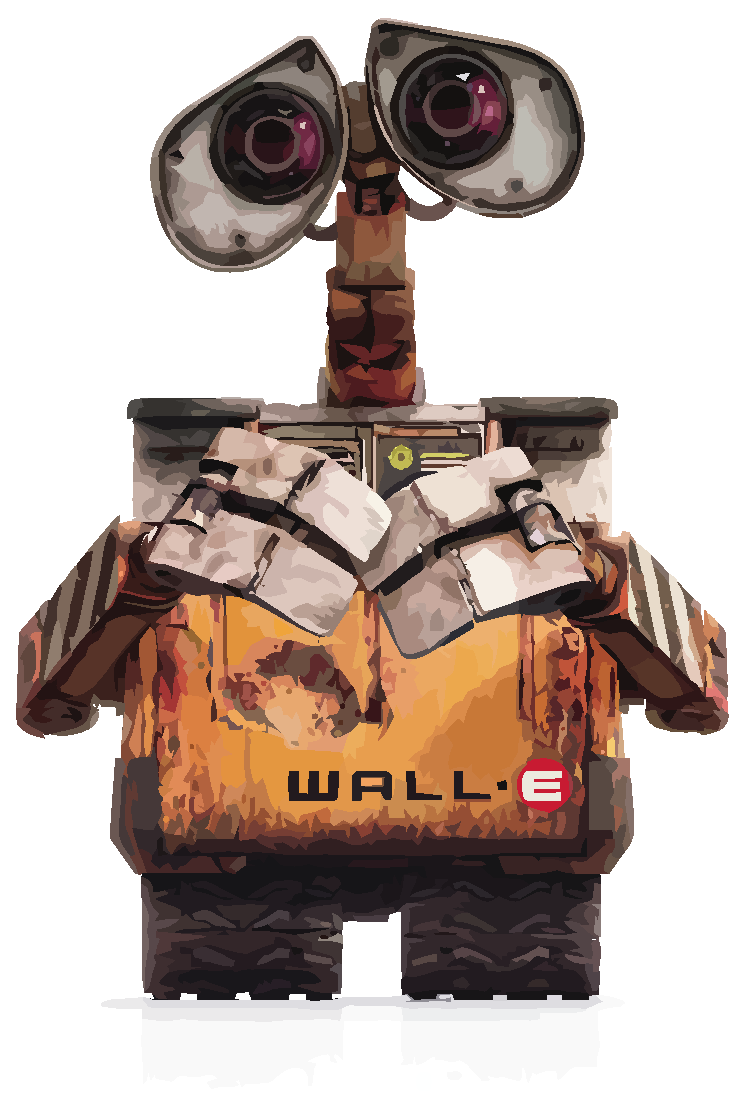
\includegraphics[width=\textwidth]{WallE}
%     \caption{Wall-E}
%     \label{fig:WallE}
%   \end{subfigure}             
%   \begin{subfigure}[b]{0.3\textwidth}
%     
\includegraphics[width=\textwidth]{minion}
%     \caption{Minions}
%     \label{fig:Minnion}
%   \end{subfigure}
%   \caption{Best Animations}
%   \label{fig:animations}
% \end{figure}


% \end{landscape}

\section{Notation}
\label{sec:defGeneral}
We use the following notation throughout the thesis:
\begin{description}
\item[Vectors, Matrices] We denote column vectors by standard vector notation
  (e.g., \(\vec{x}, \vec{y}\)) and matrices by bold upper-case letters (e.g.,
  \(\mathbf{A}, \mathbf{B}\)). We write \(\vec{b}^{T}\) to convert a vector
  \(\vec{b}\) into a row vector. The length of a vector
  \(\vec{b} = [b_{0}, b_{1}, \dots, b_{n-1}]\) (\textit{norms}) is denoted by
  \(\norm{\vec{b}} = \sqrt{b_{0}^{2} + b_{1}^{2} + \dots + b_{n-1}^{2}}\) for
  Euclidean norm and \(\norminf{\vec{b}} = max(|b_{i}|)\) for infinity norm. The
  \(i\) component of a vector is denoted interchangebly as \(b_{i}\) or
  \(b[i]\).
\item[Groups and Rings] Sets of numbers are denoted as standard (e.g.,
  \(\mathbb{R}\) for the set of rational numbers, \(\mathbb{Z}\) for integers), we
  denote \(\mathbb{Z}_{q}\) to be the set of integers modulo \(q\) (in the range
  \((-q/2,q/2]\)).\(\mathbb{Z}[n]\) denotes polynomials of order \(n\) with
  elements in \(\mathbb{Z}\), \(R_{q}\) denotes the ring of polynomial modulo
  \(x^{n} + 1\): \(R_{q} = \frac{\mathbb{Z}_{q}[x]}{x^{n} + 1}\). We use bold
  lower-case to denote an element of the ring \(R_{q}\) (e.g.,
  \(\mathbf{a} \in R_q\)).
\item[Others] We use notation \(x \randomsample D\) when \(x\) is sampled
  uniformly random from the distribution \(D\). If \(x\) is the output of an
  algorithm \(D\), we write \(x \gets D\). Algorithms are \(efficient\) if they
  run in probabilistic polynomial time (PPT). A function is said \(negligible\)
  in \(n\) if it vanishes faster than the inverse of any polynomial.
\end{description}

\section{Lattices}
\label{sec:defLattices}

\subsection{Motivation}
\label{ssub:The motivations}
We choose lattice-based cryptography as the main techniques used in the
thesis for several reasons:
\begin{description}
\item[Provable Security.] Lattice-based cryptosystems' security can be related
  to known computationally hard problems such as the Shortest Vector Problem (SVP)
  or the Closest Vector Problem (CVP) and therefore allow to demonstrate the security
  property in terms of mathematical proofs. For classical systems such as RSA,
  there is no proof showing that breaking RSA is as hard as factoring an integer,
  even though in many cases the best attack we are aware of is to carry out an operation of this type.
\item[Quantum Resistance.] In 1994, Shor \cite{shor1994algorithms} showed that
  we can write a program for quantum computers to factor a large integer
  into prime factors.The latest D-Wave systems initial deployments show that the
  idea is feasible in near future. If this happens, it has significant
  implications for the currently used public key cryptosystems such as RSA, which
  will be broken. Lattice based cryptography is currently one of the best
  candidates to resist even quantum attacks.
\item[Homomorphic Operations.] Finally, lattice-based cryptography allows us to
  perform operations unfeasible before, namely,computing on encrypted data. This
  special type of processing is able to protect privacy in online
  communication.
\item[Research Progress.] Research on Lattice-based systems has been promoted actively
  in the last decade and has reached a stage allowing for
  implementation in a near future.
\item[Performance.] Lattice-based cryptography has the potential to achieve very
  fast operations and is therefore a good option for high-performance requiring
  cryptographic applications.
\end{description}
We will recall some of the mathematics behind lattices (lattices are actually
mathematical objects). We will look into the definitions and take some of the core
problems underpinning security into consideration, focusing on how to use lattices to build
cryptographic schemes.


% In terms of efficiency, a brief summary is as follows
% \begin{itemize}
%     \item RSA - key length $\tilde{O}(n^3)$, computation $\tilde{O}(n^6)$.
%     \item ECC - key length $\tilde{O}(n)$, computation $\tilde{O}(n^2)$.

% \end{itemize} The comparison was done on some public key cryptosystems, for RSA,
% for example if we want security level of $2^n$.That means any attack on the
% system will need to run in the order of $2^n$ steps.  Then we can try to measure
% what size of key do we need, and how much computation we need to encrypt. For
% RSA, it’s 6th degree polynomial for computation, that increases quickly with n.
% Even for ECC, the key length is the best we can hope for O(n), the computation
% is still quadratic.  The good thing about lattice based cryptography is we can
% reduce both of the key length and the computation at least in the theoritical
% sense, in the asymptotic sense, when n grows to large values, both key length
% and computation grow linear with $O(n)$. In practice, it’s not as good as
% expected.  But it still quite good, for example if we need n ~ 100 bits of
% security, then in terms of computation, we can have cryptosystem that are 100
% times faster than RSA, and  the key length is a bit bigger than RSA. In
% practice, the advantage of lattice based cryptography is the speed of the
% computation rather than the length of the key.

% Regarding provable security, we can say lattice based cryptography starts from
% 1978 when all of the public key started. The Knapsack cryptosystem is worth
% mentioned here as researchers did spend a lot of effort on improving and
% breaking it, however whenever there was an improvement, then came another attack
% and the cryptosystem was never adopted. It’s not until 1996 when Ajai introduced
% the SIS problem, it’s kind of a variant of knapsack, but it came with
% mathematical proof saying that if there is any algorithm that can solve SIS,
% then we can use it to solve hard lattice problems, even worst-case instances!
% This proof make sure there is no easy way to break the cryptographic tools based
% on SIS, specifically Ajtai introduced the hash function based on SIS. It took
% another 10 years until Regev introduced the LWE problem and a cryptosystem based
% on it. And in the last 10 years, we can see that this area has been actively
% researched both in the analysis and the design of different schemes.

\subsection{Lattice Preliminaries}
\label{ssub:The mathematics}
This is an area of mathematics combining both matrices, vector algebra
and integer variables. The definitions include:

\begin{definition}[Lattice]
  An n-dimensional (full-rank) \emph{lattice} $L(B)$ is the set of all integer
  linear combinations of some \emph{basis} set of linearly independent vectors
  $\vec{b_1},\dots,\vec{b_n} \in \mR^n$:
  \[
    L(B) = \left\{ c_1 \vec{b_1} + c_2 \vec{b_2} + \dots + c_n \vec{b_n} : c_i
      \in \mZ, i = 1, \dots, n \right\}
  \]
  The $ n \times n$ matrix $B = (\vec{b_1},\dots, \vec{b_n})$ is called a basis
  for $L(B)$. There are infinitely many different bases for a lattice.
\end{definition}

\textbf{Example.} Consider a 2-dimensional lattice generated by the basis
$(\vec{b1}, \vec{b2}) = \left( \begin{bmatrix} 1 \\ 2
  \end{bmatrix} \begin{bmatrix} 0 \\ 3
  \end{bmatrix}\right)$
\begin{figure}[h]
  \centering 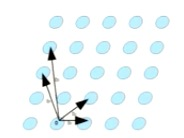
\includegraphics{lattices}
  \caption{Example of a 2-dimensional lattice}
  \label{fig:2dimLattice}
\end{figure}
To generate a lattice from a basis, we compute all the integer multiples of
each vector of the basis, then we add them together to generate new vectors. The
result is an infinite grid of vectors, this grid is a lattice. We can illustrate
two or three dimensional lattices easily, for higher dimensions, it is not
possible to draw them, but the intuition stands and all 
algebraic operations can be performed easily on the coordinates of the vectors. In
lattice-based cryptography, we work with high dimensional lattices ($n > 100$) for
security reasons. In fact, we can also say that a lattice is an infinite
group (a group is a mathematical structure, a set with a single operation on it),
the main one being addition.

\begin{definition}[Fundamental Paralellepiped]
  For an n-dimensional lattice basis
  $B = \left( \vec{b_1}, \dots, \vec{b_n} \right) \in \mR^{n \times n}$, the
  \emph{fundamental paralellepiped} (FP), denoted $P(B)$, is the set of all real
  valued $[0,1)$-linear combinations of some basis set of linearly independent
  vectors $\vec{b_1}, \dots ,\vec{b_n} \in \mR^n$.
  \begin{figure}[h]
    \centering 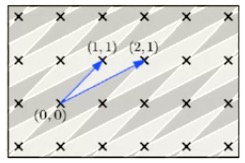
\includegraphics[scale=0.7]{parallelopiped}
    \caption{A paralellogram of 2-dimentional lattice}
    \label{fig:paralellopiped}
  \end{figure}
\end{definition}
In order to determine if a set of vectors is a basis of a lattice, there are
geometric and algebraic approaches.
\begin{lemma}
  There is exactly one \emph{L} point contained in P(B') (the $\vec{0}$ vector)
  if and only if B' is a basis of L.
  \label{lem:parallelopiped}
\end{lemma}
\begin{lemma}
  B' is a basis of L(B) if and only if B'=B.U, for some $n \times n$ integer
  matrix U with $det(U) = \pm 1$, such U is called unimodular matrix.
  \label{lem:detBasis}
\end{lemma}
$det(U)$ denotes the determinant of the matrix $U$.  Geometrically, the
determinant computes the area (or volume) of the paralellogram of a lattice. We
can associate each point of a lattice with a paralellogram; consequently, for a
large n-dimensional ball $S$, the number of lattice points in $S$ is
$\approx vol(S) / det(L)$.
\begin{definition}[Determinant]
  \label{def:determinant}
  For an n-dimensional latice $L(B)$, the determinant of $L(B)$, denoted
  $det(L(B))$ is the n-dimensional volume of the FP P(B).
\end{definition}
\begin{lemma}
  For an n-dimensional lattice $L(B)$, we have $det(L(B)) = |det(B)|$.
  \label{lem:determinant2}
\end{lemma}
Cryptography involves handling of computationally complex problems. Some are related to the geometry of lattices, such as the Shortest
Vector Problem (SVP) and the Closest Vector Problem (CVP).
\begin{definition}
  For an n-dimensional lattice $L$, its \emph{minimum} $\lambda(L)$ is the
  length of the shortest non-zero vector of $L$:
  \[
    \lambda(L) = min(\norm{\vec{b}}: \vec{b} \in L \ 0
  \]
  \label{def:minLattice}
\end{definition}
\begin{theorem}
  [Minkowski's First Theorem] For any n-dimensional lattice $L$, we have
  $\lambda(L) \leq \sqrt(n).det(L)^{1/n}$.
  \label{the:minkowski1}
\end{theorem}
As mentioned, the problem of finding SVP of a lattice becomes harder as the dimensions
grow: in theoretical computer science, this problem is categorized as
NP-hard. In cryptography, we do not use SVP as it is, we use a variant of the
problem, the definition of approximate SVP problem $\gamma-SVP$, defined below.
\begin{definition}
  [$\gamma$-SVP problem] Given a basis $B$ for an n-dimensional lattice $L$,
  find $\vec{b} \in L$ with $0 \leq \norm{\vec{b}} \leq \lambda(L)$.
  \label{def:gammaSVP}
\end{definition}
As $\gamma$ increases, the problem becomes easier. We have good algorithms to
find $\gamma$-SVP as follows
\begin{itemize}
\item For $\gamma \geq 2^{O(n)}$: LLL algorithm solves in Poly(n) time.
\item For $\gamma \leq O(1)$: NP-hard, it is not likely that a Poly(n) algorithm to solve the problem exists.
\end{itemize}
In cryptography, many systems depend on this $\gamma$-SVP problem, where
$\gamma$ is in between the two extremes $\gamma \approx O(n^c)$. Even with this
factor, the best algorithm (including quantum ones) still takes $2^{O(n)}$ time
to solve $\gamma$-SVP. ( In classical cryptosystems for example RSA, the best
algorithm to solve the integer factorization problem takes
$\approx O(2^{n^{1/2}})$ time, this is why we need a 4096 bits key to obtain
about 64 bits of security for lattices).

\subsection{q-ary lattices and SIS problem}
\label{sub:q-ary lattices and SIS problem}
There are many useful subclasses of special lattices. In cryptography, we often
use one of these, called \emph{q-ary} lattices, which relate to a problem termed
Short Integer Solution - SIS (This is a hard problem used in many cryptographic
design solutions, our ZKP technique is also based on a variant of this problem). Recall
that our motivation for lattice-based cryptosystems is the hardness of the
$\gamma-SVP$ problem given a basis $B$. It is critical to initially chose the
basis $B$ to make sure that solutions to the challenges it gives rise to are hard to find,as
there are easy instances of $\gamma-SVP$, even for $\gamma=1$. We thus need a way to
generate \emph{random} lattices' bases for which $\gamma-SVP$ is hard to solve
'on-average'. One possible answer comes from \cite{ajtai1996generating}: random
\emph{q-ary} lattices, for which the hardness of finding short
vectors within them can be proved.

\begin{definition}[Ajtai's perp lattices]
  Given an integer \emph{q} and a uniformly random matrix
  $A \in \mathbb{Z}_{q}^{n \times m}$, the \emph{q-ary} perp lattice
  $L_q^\bot(A)$ is defined by:
  \[
    L_q^\bot(A) = \left\{ \vec{v} \in \mathbb{Z}^m : A.\vec{v} = \vec{0} \mod \
      q \right\}
  \]
\end{definition}
Although it might not be clear from the aforementioned definition of lattices, the set of all vectors
$\vec{v}$ actually forms a lattice. They can be generated by some basis, and
there is a fast algorithm to compute such basis. The parameters for these
lattices are $A$ and $q$ and we can choose a lattice to work on by selecting random
values for these parameters. This particular set of \emph{q-ary} lattices is convenient
because Ajtai mathematically proved that If there is an algorithm to break the
$\gamma-SVP$ problem for these lattices, we could use the same algorithm to break
$\gamma-SVP$ for any lattice. This is the \emph{worst-case to average-case}
security reduction and gives us confidence in concluding that the problem is hard on average.
\begin{definition}[Small Integer Solution (SIS) problem]
  $SIS_{q,m,n,\gamma}$ Given n and matrix $A$ sampled uniformly in
  $\mathbb{Z_q^{n \times m}}$, find $\vec{z} \in \mathbb{Z}^{m \times n}$ such
  that $A\vec{v} = \vec{0}$ and $\norminf{v} \leq \beta$.
  \label{def:SISProblem}
\end{definition}
Informally, SIS is just the name given to the $\gamma-SVP$ problem for the
particular \emph{q-ary} lattices. $\beta$ is the approximation parameter, it
tells us how short the lattice vector should be. Some relations between SIS and
$\gamma-SVP$:
\begin{itemize}
\item $det(L_q^\bot(A)) = q^n$
\item By Minkowski's Theorem, $\lambda(L_q^\bot(A)) \leq \sqrt{m}$, for
  $m \geq n \log q$. So to solve SIS, we need to find vectors not much longer
  than $\sqrt{m}$.
\item We can relate $\gamma$ of SVP to $\beta$ of SIS:
  $\gamma \approx \beta/\sqrt{m}q^{n/m}$.
\end{itemize}

\subsection{A cryptographic example}
\label{sec:ajtaiHash}
Cryptographic hash functions have many applications to
provide authenticity and integrity in different security contexts. One of the main properties of cryptographic
hash functions is collision resistancy: it is hard to find 2 message inputs
producing the same hash value output. The current constructions being used in practice
are not lattice-based but based on non-linear boolean functions. We discuss how
to construct a variant from lattices and show the relevant techniques
to be used during security proofs and parameter choices throughout this
thesis. The security level of this function is directly related to the hardness of
the SIS problem pointed out before
\begin{definition}[Ajtai's Hash Function.]
  Pick $A=(\mathbf{a_{i,j}}) \randomsample \mathbb{Z}_q$ ($A$ is the function
  'public key'). Given $\vec{x} \in \mathbb{Z}^{mn}$ having 'small' coordinates
  ($\norminf{\vec{x}} \leq d$), the hash function out put is defined as
  \[
    g_{q,m,n,d,A}(\vec{x}) = A . \vec{x} \mod \ q
  \]
  \label{def:Ajtai's Hash Function}
\end{definition}
We can see here that from a long input vector, we obtain a short output vector, which is
our hash value. The parameter values should be chosen so as to make sure that the collision resistance constraint is
satisfied. The important question is how to determine the security of this
function, or how to ensure that this function is collision resistant. To this end, we
introduce the concept of security reduction, used frequently in
lattice-based cryptography's security proofs. We show that if there
was an algorithm to find a collision in this hash function, then we could use
such an algorithm to solve a hard lattice problem. In our case, we know that SIS
was analyzed by Ajtai and shown to be hard, based on good foundations. What we
are going to show here is that, if we can find a collision efficiently in this hash
function, we could also efficiently find a way to break the SIS problem, which
would contradict the hardness of SIS. Elaborating on this contradiction, we can
conclude that there must not exist any efficient algorithm to find collision for
the hash function.
\begin{theorem}
  Collision-Resistance of $g$ is at least as hard as $SIS_{q,m,n,\beta}$ with
  $\beta = 2d$.
  \label{the:ajtai hash}
\end{theorem}
\begin{proof}
  Suppose there was an efficient collision-finder attack algorithm $CF$ for
  function $g$: Given a random instance $(A,q)$, $CF$ outputs
  $\vec{x_1} \neq \vec{x_2}$ such that $A\vec{x_1} = A\vec{x_2}$.

  We then can use $CF$ to build another algorithm $S$ that solves SIS problems
  for any instance $(A,q)$:
  \begin{itemize}
  \item Runs $CF$ on $(A,q)$ to get $\vec{x_1},\vec{x_2}$.
  \item $S$ outputs solution for SIS problem: $\vec{v} = \vec{x_1} - \vec{x_2}$.
  \end{itemize}

  The algorithm works because $A\vec{v} = A\vec{x_1} - A\vec{x_2} = \vec{0}$,
  i.e., $\vec{v}$ is in the lattice $L_q^\bot(A)$ and
  $\norminf{\vec{v}} \leq \beta$, where $\beta = 2d$ (When we add/substract
  vectors ,the result vector's length is upper bounded by the sum of the lengths
  of the vectors). Moreover, $S$ is efficient as $CF$ is efficient (run-time
  $T_S \approx T_{CF})$.
\end{proof}
This has been the first application of lattices in cryptography and it actually
triggered other modern techniques. The next important questions are
\begin{itemize}
\item How should we choose the parameters to obtain a given security level?
\item How to secure is SIS problem related to $\gamma-SVP$ problem?
\end{itemize}

\subsection{Security of lattice-based cryptography}
\label{sec:latticeSecurity}
Lenstra–Lenstra–Lovász (LLL) and its various improvements are the main ways to
access the security of lattice-based systems (by accessing the security of
underlying problems, such as SVP .or $\gamma-SVP$). From there, it allows us to
choose the size of the parameters for the problem at hand (such as dimensions), in order
to provide guarantee of security against the best known attack.

We first recall an important concept related to lattices, used in LLL:
Gram-Schmidt Orthogonization (GSO)
\begin{definition}
  [GSO] For a lattice basis
  $B = \left( \vec{b_1}, \vec{b_2}, \dots, \vec{b_n} \right)$, its GSO is the
  matrix of vectors
  $B^* = \left( \vec{b}_1^*, \vec{b}_2^*, \dots, \vec{b_n^*} \right)$ defined by
  $\vec{b_1^*} = \vec{b_1}$ and for $i \geq 2$,
  $\vec{b_i^*} = \vec{b_i} - \sum_{j=1}^{i-1}{\mu_{i,j}.\vec{b_j^*}}$, where
  $\mu_{i,j} = \frac{\langle \vec{b_i}, \vec{b_j^*} \rangle}{\langle
    \vec{b_j^*},\vec{b_j^*} \rangle}$.
  \label{def:GSO}
\end{definition}
GSO is basically a way to convert a basis that we have (that are not orthogonal)
into another set of vectors are orthogonal. Figure \ref{fig:gso} shows an
example of GSO in 2-dimensional
\begin{figure}[h]
  \centering 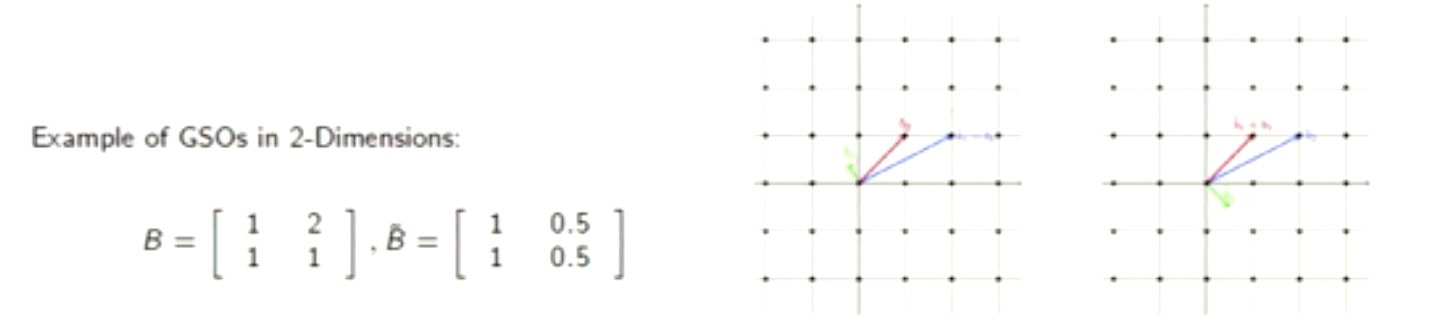
\includegraphics[scale=0.3]{gso}
  \caption{Example of GSO in 2-dimensions}
  \label{fig:gso}
\end{figure}
GSO is used as part of the LLL algorithm to find short vector of a lattice.
Note that the $GSO(B)$ is not another basis for the original lattice, it is just
a related matrix, it has the same determinant as the original one.

% Once we have done the transformation from $B$ to $B^* = GSO(B)$, we can also
% write the relation between the two of them algebraically as in Figure \ref{}
% \begin{figure}[h]
%   \centering 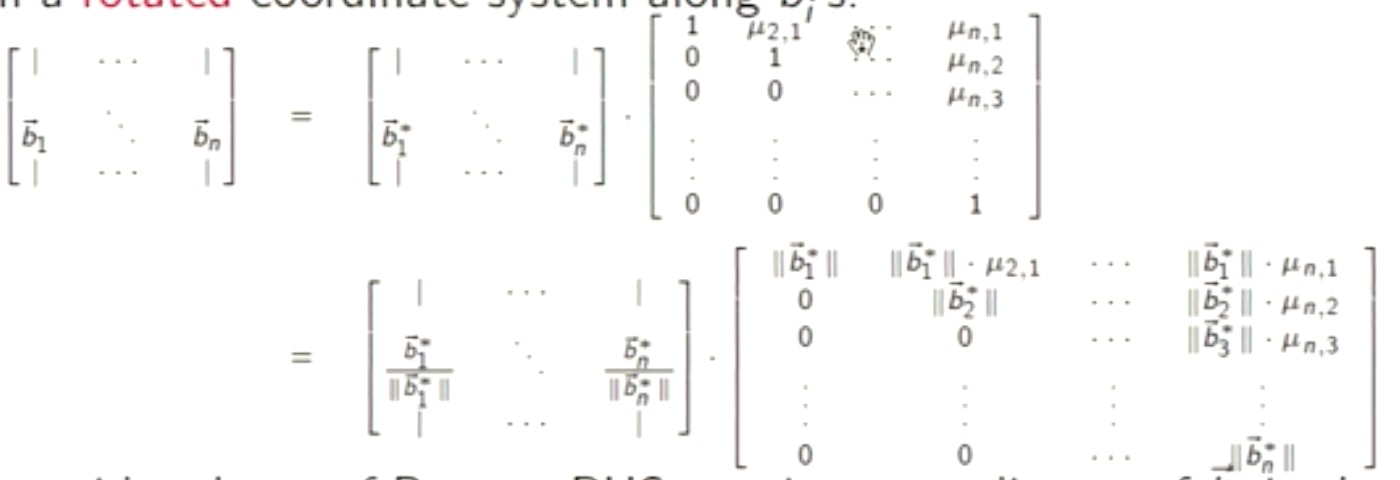
\includegraphics[scale=0.3]{gsoMatrix}
%   \caption{GSO algebraic relation}
%   \label{fig:GSOAlgebra}
% \end{figure}
% We can intepret the second relation as a rotated coordinates system. Another
% nice observation we can have from this matrix representation is the 0s in the
% matrix implies the determinant of the lattice:
% \[
%   det \ L(B) = |det(B)| = |det(B^*)| = \prod_{i=1}^{n}\norm{\vec{b_i^*}}
% \]

% Back to our LLL discussion, this is the main algorithm to find short vectors in
% lattices, and therefore the main type of attack against lattice-based
% cryptosystems in practice, the other approach is exhaustive search. The best
% algorithm is the combination of the 2 approaches to trade off the runtime verse
% the approximation factor. We will discuss this algorithm (BKZ) in a later
% section.

\subsubsection{LLL algorithm}
\label{sec:LLLalgorithm}
The Lenstra–Lenstra–Lovász (LLL) algorithm not only finds short vectors but also
manipulates the basis of the lattice into another basis of the lattice. Given
some basis as an input to LLL (whose vectors are long), LLL makes sequential
modifications to it, every modification still keeping it as the basis of the
lattice but slightly improving it. As the improvements repeat, the sizes
of the vectors of the basis are reduced, until a matrix that
cannot be improved anymore is obtained. That is the output of LLL: a basis of the lattice
much better than the original input, in the sense that it has much
shorter vectors.

In more detail, LLL looks at the property of the GSO of the basis to make its vectors 'approximately' orthogonal. The size of the GSO basis tells us the
length of the projections of one vector along the earlier vectors. The larger
these are, the less orthogonal the basis vectors are, because they have bigger
components along the earlier vectors. LLL tries to reduce those coefficients
(projection coefficients), to make them more orthogonal, which will also make
them shorter. There are 2 tests that LLL performs to define how orthogonal the basis
vectors are

\begin{description}
\item [LLL property 1.] Takes the current basis of the lattice and computes the
  GS coefficients $\mu_{i,j}$. It checks $|\mu_{i,j}| \leq 1/2$, that is, the
  length of the projections on the previous vectors are at most half of the
  actual full vector. If this condition is not satisfied, LLL modifies the basis
  until the condition obtains.
\item [LLL property 2.] The algorithm looks at the large remaining component
  $\norm{\vec{b_{i+1}^*}}$ of $\vec{b_{i+1}}$ after removing components along
  $\vec{b_j^*}$'s ($j < i + 1$) and checks
  \[
    \norm{\vec{b_{i+1}^*}+\mu_{i+1}\vec{b_i^*}}^2 \geq \delta
    . \norm{\vec{b_i^*}}^2
  \]
  for all $i=1,\dots,n-1$ and for some constant
  $\delta$($1/4 \leq \delta \leq 1$).

  Informally, the second check is a bit more complex: LLL looks at the last 2
  components of each vector, such as $\vec{b_i}$, and decomposes it
  into all the projections along the previous $\vec{b_j^*}$. It then checks the 
  sum of the current orthogonal component against the the sum of the previous orthogonal component (for example, if
  we look at $\vec{b_{i+1}}$, we check
  $\norm{\vec{b_{i+1}^*}+\mu_{i+1}\vec{b_i^*}}^2$). If this quantity is big
  enough, it points at the fact that we have a lot left over after removing the
  components along the previous one. The bigger this length, the more
  orthogonal the basis becomes. The algorithm tries to make it big enough. The
  parameter $\delta$ of the algorithm defines this magnitude (the larger
  $\delta$ is, the better the result returned by the algorithm).

  This check is carried out for all the vectors of the basis. If it is not
  satisfied, then  LLL does some new changes to make sure the test passes.
\end{description}

When the algorithm runs, the 2 checks keep competing with each
other. The algorithm is designed to run until reaching the stage where both of the checks satisfy
simultaneously and to output the new basis after that.(Algorithm
\ref{alg:LLL})
\begin{definition}
  A basis $B$ for lattice $L$ is $\delta-LLL$ reduced if both LLL properties 1
  and 2 are satisfied.
  \label{def:LLL}
\end{definition}

\begin{algorithm}
  \caption{LLL algorithm}
  \label{alg:LLL}
  \begin{algorithmic}[1]
    \Procedure{LLL}{$B$} \State Compute GSO $B*$ for B.  \For {$(i=2,\dots,n)$}
    \For {j = i - 1 to 1} \State
    $c_{i,j} \gets \lceil{\frac{\langle \vec{b_i}, \vec{b_j^*} \rangle}{\langle
        \vec{b_j^*},\vec{b_j^*}\rangle}}\rfloor$ \State
    $\vec{b_i} \gets \vec{b_i} - c_{i,j}\vec{b_j}$ \EndFor \EndFor \If
    {$\norm{\vec{b_{i+1}^*}+\mu_{i+1}\vec{b_i^*}}^2 \geq \delta
      . \norm{\vec{b_i^*}}^2$} \State Swap $\vec{b_i}$ and $\vec{b_{i+1}}$.
    \State Go back to step 2.  \Else \State Return B \EndIf \EndProcedure
  \end{algorithmic}
\end{algorithm}
Note that in the algorithm we take the rounded multiple of $\vec{b_j}$, this
important operation causes the algorithm to maintain the vectors as the basis of
the lattice. As the lattice consists of only integer multiples of all the basis
vectors, when adding an integer multiple of $\vec{b_j}$ to $\vec{b_i}$, we still
end up with another lattice vector. We can also show that the new matrix is also
a basis of the lattice. In other words, if we add a fraction of $\vec{b_j}$, it is
not a lattice point anymore. Also, due to this rounding error, instead of having 
precisely orthogonal vectors in the result matrix, we only obtain an approximate
orthogonal matrix. For an intuitive comprhension of the algorithm, we refer the reader to
\cite{lenstra1982factoring}. Last but not least, the loop of the algorithm consistently succeeded in terminating in polynomial time!
\begin{theorem}
  [LLL run time] The number of iterations of LLL on an input basis B before
  termination is at most
  \[
    n^2.\log{(\max{\norm{\vec{b_i}}})} / \log{(1/\sqrt{\delta})}.
  \]
  For any constant $1/4 < \delta < 1$, this is polynomial in bit length of the
  algorithm input. Moreover, the run-time for each iteration is also polynomial
  in the input bit length. Overall, run-time is polynomial in input length, or
  LLL is efficient!
  \label{theo:LLLRunTime}
\end{theorem}

\subsubsection{LLL solution to $\gamma-SVP$}
\label{sec:LLLsolution}
The question is how short the vectors of LLL's output are, or what kind of
approximate SVP LLL is able to solve: If we run LLL on some basis, we get back a
reduced basis, and we take the shortest vector in that result basis. How long is
that vector compared to the shortest vector in the lattice.
\begin{theorem}
  [Short vector from LLL]. The LLL algorithm solves in polynomial time
  $\gamma-SVP$ for $n-dim$ lattices, with $\gamma < 2^{(n-1)/2}$.
  \label{theo:LLLShortVector}
\end{theorem}

% \begin{proof}
%   The idea is to combine both of the relations in LLL to show that if we take
%   the ratio of the length between to successive Gram-Schmidt vectors of the
%   lattice: $\frac{\norm{\vec{b_{i+1}^*}^2}}{\norm{\vec{b_i^*}^2}}$, it is always
%   going to be at least $(\delta - 1/4)$. It means that when we go from $i$ to
%   $i+1$, the length of $\vec{b_i^*}$ cannot decrease by more than a factor of
%   2. After $n$ steps, the length drops $2^n$ times. One of the property of the
%   Gram-Schmidt basis mentioned was: the last Gram-Schmidt's vector length is a
%   lower bound of the length of the shortest vector in the lattice: $\vec{b_1^*}$
%   is always less than the length of the shortest vector of the lattice. Since
%   $\norm{\vec{b_1^*}}$ can only be at most \todo[inline]{finish proof}
% \end{proof}

In summary, the first vector of LLL output is bounded by
\[
  \norm{\vec{b_1^*}} \leq (1/(\delta-1/4))^{(n-1)/2}.\lambda(L)
\]
% The $\delta$ parameter of the algorithm therefore also contribute to
% the output.
We can see that the approximation factor is exponential in the dimention $n$ of
the lattice. Another way to measure the length of the output vector of LLL is the Hermite
Factor (HF), which is the ratio of the algorithm's output to the $n^{th}$ root
of the determinant of the lattice. Sometimes it is more convenient to use this
measure because the determinant of the lattice is easy to compute,
whereas the length of the shortest vector of the lattice is not, in general. In
practice we usually use this as a main measure. Again, LLL gives HF that is
exponential in the dimension $n$. The conclusion is, although LLL runs in
polynomial time, the approximation factor increases exponentially fast with
the dimension. When the dimension is large, the approximation factor will grow
so fast that LLL is not useful to break the security of underlying
cryptosystems.
\begin{theorem}
  The LLL algorithm solves in polynomial time $\gamma-SVP$ for $n-dim$ lattices,
  with $\gamma \leq 2^{(n-1)/2}$. Can also be shown that Hermite Factor
  $\gamma_{HF} = \frac{\norm{\vec{b_1}}}{det(L)^{1/n}} \leq 2^{(n-1)/4}$
  \label{theo:LLLHF}
\end{theorem}

\subsubsection{LLL in practice}
\label{sec:LLLinPractice}
This section discusses the trade-off between the running time and the length of
the output of the attack. This helps us in selecting parameters for
state-of-the-art lattice attack

In practice, we try to improve this bound so that LLL can get a shorter vector. One way
to do that is to use the fact that, in our approach, we apply worst-case analysis
on the output that LLL can give. Generally, they tend to be shorter than
that. When running LLL experimentally (\cite{nguyen2006lll}) on a random lattice, we
will notice that it performs much better than the bound proved. Specifically, $HF$
is close to $1.02^{n-1}$. Although this factor is still exponential in dimension
$n$, this slow growth allows LLL to be used with large dimension lattices. In
order to reduce this $HF$ further, LLL can be modified. There are several
ways to do that. The basic idea is to combine LLL with an exhaustive search
(enumeration algorithm). The best lattice exhaustive search algorithm
(Fincke-Phost/Kannan) does it in time $2^{O(n\log(n)}$, it is even worse than
exponential. There are variants of such a method, but they all take at least
exponential time with respect of the dimension $n$ (with the expense of using $2^{O(n)}$
memory). In general, all enumeration algorithms are very inefficient. Therefore,
combining LLL with bruteforcing is a more practical approach: BKZ is the typical
algorithm in this category.  BKZ allows trades off between run-time and
approximation factor $\gamma$, LLL is modified by changing the blocksize $k$ of
vectors in the swapping step. As we increase $k$: We search in the lattice of
dimension $k$ using brute force search and then run LLL with a smaller k dimension. We get the 'interpolation' between the two extremes of LLL (corresponding to
$k = 2, \gamma = 2^{O(n)}, T = n^c$) and the enumeration (corresponding to
$k = n, \gamma=1, T = 2^{O(n\log(n)}$)). In between, BKZ can achieve
$\gamma(k) \leq k^{(n-1)/(k-1)}$ with running time
$n^c.k^{O(k)}$. \cite{hanrot2011terminating}. From this trade-off setting, an
attacker then can choose the optimal value of $k$ for some particular context: A
lattice-based cryptographic scheme can only be broken if the adversary can find
short enough vectors. This also tells us how small $\gamma$ needs to be in order
to resist such an attack.

In summary, given a security level $\lambda$ for a system (i.e., it would take
time $2^\lambda$ for the best attack to work even with the best choice for the BKZ
parameter $k$), the best approximation factor $\gamma$ that the
algorithm can reach is related to $\lambda$ as:
\[
  \log(\gamma_{HF}) = \Omega(\frac{n\log^2\lambda}{\lambda})
\]
where $\Omega$ represent the asymptotic ``lower than'' condition when the parameters
are large. Overall, we can conclude the \emph{lattice 'rule of thumb'} for
$\gamma-SVP$ using BKZ is:
\[
  n = \Omega(\frac{\lambda}{\log^2\lambda}.\log\gamma_{HF}) \approx \lambda
  . \log\gamma_{HF}
\]

\begin{remark}
  The dimension $n$ of a lattice-based cryptosystem needs to be proportional to
  the product of bit-security level $\lambda$ and the $\log$ (base 2) of the
  approximation factor $\gamma_{HF}$.  This factor is a reason behind the long
  keys of such cryptosystems.
  \label{rem:dimension}
\end{remark}

For concrete values of parameters, Chen and Nguyen \cite{chen2011bkz} gave
numerial estimates for the Hermite Factor and time for random lattices versus block
size for optimized BKZ variant:

\begin{figure}[h]
  \centering 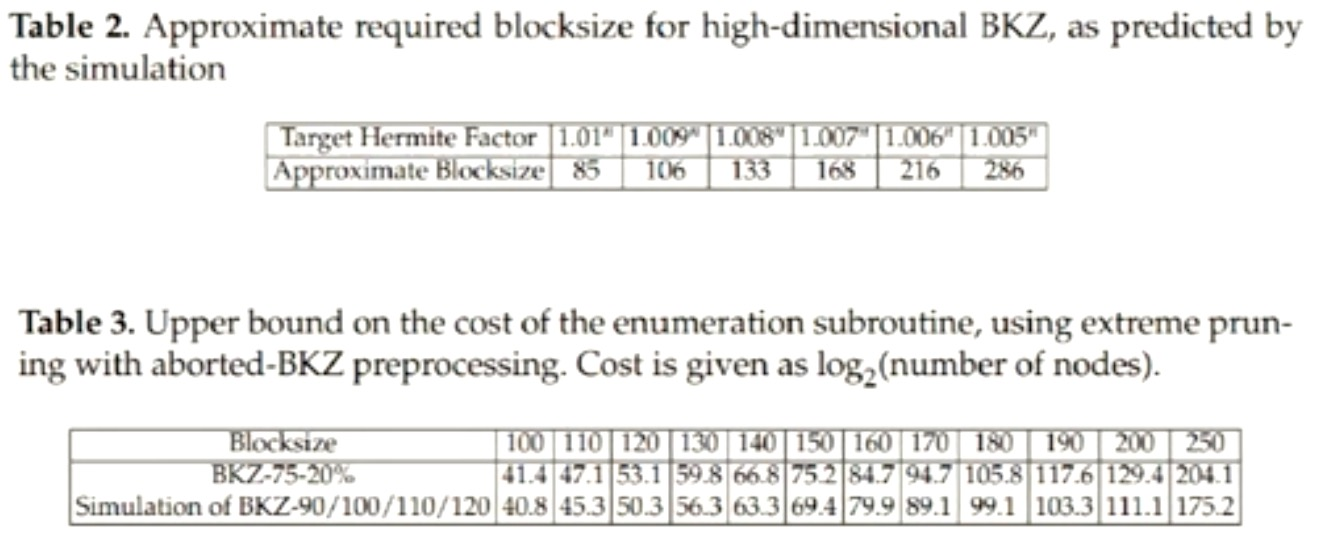
\includegraphics[scale=0.3]{bkzparams}
  \caption{BKZ parameters}
  \label{fig:BKZParams}
\end{figure}

From table 2, for a given $HF$ that we want BKZ to achieve, it gives us the
block size parameter $k$ that needs to be used. Note that the $HF$ is much
smaller than what we had for LLL (whose $HF \approx 1.02^{n-1}$ in
practice). Once we have the block size, we can look it up in table 3 to know the
running time of the algorithm.

\subsection{An example of parameter values choice}
\label{sec:parameterChoice}
We discuss Ajtai's hash function as an example of how to choose parameter values for
a given security level. We showed that if there is an algorithm that can break the
collision-resistance property of the hash function, we can use it to find a
short vector of the SIS problem with length $\beta = 2d\sqrt{m}$. The question
is how to choose the values of the parameters $q,n,m,d$ for the hash function to get a
given security level $\lambda$ based on the hardness of SIS? According to the
BKZ state-of-the-art attack, to get running time of $2^\lambda$, we can use
table 3 to derive the block size and the corresponding Hermite Factor $\gamma_{HF}$.
This information allows us to know that the best attacker can compute a non-zero vector $\vec{v}$ in SIS
lattice $L_q(A)$ of norm $\leq l = min(q, \gamma_{HF}.det(L_q(A))^{1/m})$. 
Comparing $l$ with $\beta$ (or $2d\sqrt{m}$), if $l < \beta$, predicts the success or the failure of a possible attack.

There are often ways to optimize such attacks, as the attacker can choose parameter values allowing him to minimize effort. For example in the attack of the SIS problem mentioned in
\cite{micciancio2008lattice}, the attacker can look at a subset $m' \leq m$ of
columns of $A$, finding a short vector $\vec{v'}$ such that
$A'\vec{v'} = \vec{0} \mod \ q$. He can choose $\vec{v''} = \vec{0}$ and set
$\vec{v} = \vec{v'} + \vec{v''}$. It turns out that there are optimal values an attacker can choose for $m'$ that minimize the length $l(m')$ for
$\vec{v'}$.  Specifically, $l(m') = min(q,\gamma'_{HF}.det(L_q(A))^{1/m'})$ is a
function of $m'$ (the graph of this function is illustrated in Figure
\ref{fig:bestAttack}).
\begin{figure}[h]
  \centering 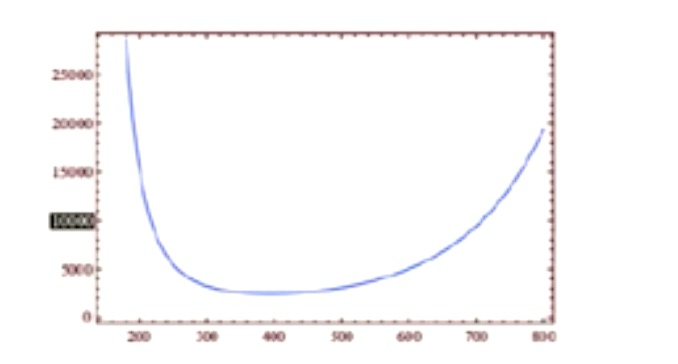
\includegraphics[scale=0.3]{bestattack}
  \caption{Choosing best m' for SIS attack for parameters
    $\delta = 1.01, q=4416857, n=100$}
  \label{fig:bestAttack}
\end{figure}
It appears that at some point $m'$ there is some minimum value for the length of
the vector we can get with BKZ, which is the value an attacker wants to
choose. Denoting $m^*$ to be this optimal selection, we have
$l(m^*) = min(q, 2^{2.sqrt{n\log q\log \delta}})$. The condition for the failure of the attack being $l(m^*) > \beta$, so
\[
  q \geq \beta = 2d\sqrt{m} \ \text{and}\ n \geq \frac{\log^2(\beta)}{\log q
    \log(\delta)}
\]
We have looked at the best practical algorithms to attack lattice problems (LLL
and its variants). In theory, there is also Ajtai's proof, where the hardness of solving the SIS problem for random matrices is addressed. The connection between average case and  worst-case complexity of lattice problems in general (lattices that are completely unrelated
to the \emph{q-ary} ones) is the theoretical foundation of lattice-based
cryptography. We present Ajtai's average-case to worst-case connection Theorem
(1996, improved by \cite{gentry2008trapdoors}).

\begin{theorem}
  [Ajtai's hardness proof for SIS.] If there is an algorithm $A$ that solves
  $SIS_{m,n,q,\beta}$ in poly-time, for some non-negligible fraction of input
  matrices $G \in \mathbb{Z_q^{m \times n}}$, then there is an algorithm $B$
  that solves $\gamma-SVP$ in polynomial time for all input lattices $L$ of
  dimension $n$ with:
  \[
    \gamma = O(\beta\sqrt{n}), q = \omega(\gamma\sqrt{\log n})
  \]
  \label{theo:AjtaiHardness}
\end{theorem}

Although the theorem does not directly yield concrete information to choose
parameter values securing a cryptosystem of the type discussed previously, it does provide  qualitative confidence in the security of the problem.

\section{Learning With Error}
\label{sub:LWE}
In the last section, we discussed how to use lattice-based cryptography to
construct a hash functions. This section looks at another main tool in
cryptography , that is, encryption, or how to ensure confidentiality. We need here to
use a type of lattice problem slightly different from the SIS problem, much more suitable for building the encryptions based on it: the Learning With Error (LWE) problem. We will discuss how to use LWE to build a symmetric key encryption as well as how to modify it to achieve public key encryption (Regev cryptosystem). This cryptosystem is foundational, as it grounds further developments in the area and techniques used in the project.

In the SIS problem, given a matrix $A$, it is asked to find a short vector
$\vec{v}$ such that $A\vec{v} = \vec{0}$. The cryptographic hash function 
 based on SIS is constructed so as to allow arbitrary inputs and
produce collision-resistance outputs. Such an architecture always implies a
many-to-one function type in the construction: given an output, the original input cannot be derived from it. This many-to-one property is not useful
in encryption contexts: we cannot decrypt the ciphertext to obtain the original
plaintext using such a method. In encryption contexts, we usually have the reverse
situation: the set of possible inputs might be a lot smaller than the set of
possible outputs. The function serving encryption should be at least a
one-to-one function that maps a plaintext to a unique ciphertext. Or we can even
have one-to-many functions mapping a plaintext to many possible ciphertexts: as
long as there is no intersection between the ciphertext output sets, we are
still able to decrypt correctly. Such situations appear in non-deterministic
cryptosystems, where the encryption function takes the message as well as a
randomness factor as inputs. Actually, almost all encryptions being used in
practice are somehow randomized, the main reason being to stop the leakage of
information given many ciphertexts. A deterministic cryptographic scheme can be
exploited if the plaintext space is small: suppose that Alice sends deterministic encrypted messages to her agent Bob everyday instructing him to sell or keep some of her companies' shares.  An attacker capturing the ciphertexts sent throughout several days can easily distinguish such decisions without having to decrypt the messages at all. This is one of the important properties that we want to include in cryptosystems: indistinguishability, also known as IND-CPA. This type of security prevents the adversary from distinguishing
the ciphertexts, even if all the possible plaintext are known.

We introduce the LWE problem \cite{regev2005lattices} allowing to construct
one-to-one or one-to-many functions. The main idea behind LWE is that, given a secret
vector and a random lattice point with some 'small noises' added to the point,
it is infeasible for an attacker to learn anything from the output, but it is
easy for the data owner with the secret to revert back to the original source. The
description of LWE follows.

\subsection{Definitions}
\label{sec:LWEDefs}
Fix integers $q, m, n$ and initialize the matrix $A^{m \times n}$. Note that the
matrix $A$ is a bit different from SIS regarding its dimension, this is just for
convenient representation purpose.  $q$ is still the modulus of $a_{i,j}$, where
$a_{i,j} \randomsample \mathbb{Z}_q$. Let
$\vec{s}^T = \left[ s_1,s_2,\dots,s_n \right]$ be a vector of independent
uniformly random elements of $\mathbb{Z}_q$, this is the secret element that
corresponds to the secret key of the cryptosystem. Let
$\vec{e}^T = [e_1,\dots,e_n,\dots,e_m]$ be a vector of independent 'small'
integers, each sampled from a probability distribution $\chi_{\alpha q}$. By
'small', we mean $\norminf{e_i} \leq \alpha . q$ for some parameter
$0 < \alpha < 1$. Typically, $\chi_{\alpha q}$ is chosen from a Normal
(Gaussian) distribution with standard deviation $\approx \alpha . q$. (From the
implementation point of view, one way to do such sampling efficiently is to take
the real samples from a normal continuous distribution and round it to the
neareast integers, the mean is set to 0 to make sure the samples are small).


We discuss two variants of the LWE problems to be used in cryptosystems:
Search-LWE and Decision-LWE problems.

\begin{definition}
  [Search-LWE Problem.] Given $q,m,n,\alpha$ and a matrix
  $A \randomsample \mathbb{Z}_q^{m \times n}$ and
  $\vec{y} = A.\vec{s} + \vec{e} \mod q$ (with
  $\vec{e} \randomsample \chi_{\alpha q}^m$ and
  $\vec{s} \randomsample \mathbb{Z}_q^n$), find $\vec{s}$.
  \label{def:Search-LWEProb}
\end{definition}

\begin{definition}
  [Decision-LWE Problem.] Given $q, m, n, \alpha$ and
  $A \randomsample \mathbb{Z}_q^{m \times n}$, $\vec{y}$, distinguish between
  the following two scenarios
  \begin{itemize}
  \item \emph{Real Scenario:} $\vec{y} = A.\vec{s} + \vec{e} \mod \ q$ (with
    $\vec{e} \randomsample \chi_{\alpha q}^m$ and
    $\vec{s} \randomsample \mathbb{Z}_q^n$)
  \item \emph{Random Scenario:} $\vec{y} \randomsample \mathbb{Z}_q^m$.
  \end{itemize}
  \label{def:Decision-LWEProb}
\end{definition}

\subsection{Security of LWE}
\label{sec:LWESecurity}
An average-case to worst-case connection similar to Theorem
(\ref{theo:AjtaiHardness}) for SIS problem can also be established for LWE
(\cite{regev2005lattices})
\begin{theorem}
  If there is an algorithm $A$ that solves $DLWE_{q,m,n,\alpha}$ in poly-time,
  with non-negligible distinguishing advantage, for $\alpha . q > 2
  \sqrt{n}$. Then there is a quantum algorithm $B$ that solves $\gamma-GapSVP$
  in polynomial time for all input lattices $L$ of dimension n with:
  \[
    \gamma = O(n/\alpha)
  \]

  \label{theo:RegevLWEHardness}
\end{theorem}
Theoretically we have strong reason to believe that LWE is hard. The theorem
even says that it links the security of LWE to the quantum security of the
shortest vector problem. It therefore gives us more confidence to use LWE as the
basis for quantum resistant cryptographic technique. In practice, the best known
attack against LWE is to reduce the problem to the SIS problem: Given a LWE
instance $(A \in \mathbb{Z}_q^{m \times n},\vec{y} \in \mathbb{Z}_q^m)$:
\begin{itemize}
\item Find a short non-zero vector $\vec{v}$ in the SIS lattice $L_q^\bot(A^T)$
  with $\norm{v} \leq \beta$. That is, $A^T.\vec{v} = \vec{0} \mod q$.
\item Compute $e' = \vec{v}^T.\vec{y} \mod q$ and check:
  \begin{itemize}
  \item In 'Real DLWE Scenario', $e'$ is small
  \item In 'Random Scenario', $e'$ is not small
  \end{itemize}
\end{itemize}

In other words, solving $DLWE_{q,m,n,\alpha}$ reduces to solving
$SIS_{q,m,n,\beta=1/\alpha}$, therefore to secure the system based on DLWE, we
must choose parameters so that $SIS_{q,m,n,\beta}$ is hard. (The smaller the
noise we choose for DLWE, the larger the $\beta$ becomes, or $\gamma-SVP$ is
easier, which is expected).  Also, the condition of $\alpha q > 2\sqrt{n}$ is
also important as when the noise become small enough, it turns out that there
are efficient algebraic attacks against LWE.

\subsection{Symmetric cryptosystem from LWE}
\label{sec:LWESymmetric}
We present a randomized cryptosystem based on LWE
\begin{description}
\item[Key Generation - KeyGen.] Fix integers $q, n$. Pick a secret key
  $\vec{s} \randomsample \mathbb{Z}_q^n$.
\item [Encryption - Enc.] Fix integers $t,l$. Given a message
  $\vec{m} \in \mathbb{Z}_t^l$:
  \begin{itemize}
  \item Pick $A \randomsample \mathbb{Z}_q^{l \times n}$ and 'small' noise
    $\vec{e} \randomsample \chi_{\alpha q}^l$.
  \item Compute
    $\vec{c} = A.\vec{s} + \vec{e} + \lceil q/t \rfloor . \vec{m} \mod \ q$.
  \item Return ciphertext $(A, \vec{c}$.
  \end{itemize}
\item [Decryption - Dec.] Given a ciphertext $(A,\vec{c})$ and a secret key
  $\vec{s}$:
  \begin{itemize}
  \item Compute $\vec{c'} = \vec{c} - A.\vec{s} \mod \ q$.
  \item Compute $\vec{c''}$ by rounding coordinates of $\vec{c'}$ to the
    neareast multiple of $\lceil q/t \rfloor \mod \ q$. This step exploits the
    fact that $\vec{e}$ is a 'small' vector rather than a random one.
  \item Return plaintext $\vec{m} = \frac{\vec{c''}}{\lceil q/t \rfloor}$
  \end{itemize}

\item [Correctness.] Decryption is correct if the rounding step succeeds, or if
  all the noise coordinates $e_i$ of $\vec{e}$ is sufficiently small:
  \[
    e_i < \frac{1}{2} . \lceil q/t \rfloor \approx \frac{q}{2t}
  \]
  If the noise distribution $\chi_{\alpha q}$ is a normal distribution with
  standard deviation $\alpha q$, the probability that the noise exceeds
  $\frac{1}{2t\alpha}$ in magnitude is
  $p_e \approx 2.\left( 1 - \Phi\left( \frac{1}{2t\alpha} \right) \right)$,
  where $\Phi$ is the cumulative distribution function of the standard normal
  distribution (mean 0 and standard deviation 1). Therefore, to assure
  correctness, we need this probability to be sufficiently small, the following
  \emph{correctness condition} must holds:
  \[
    t << \frac{1}{2\alpha}
  \]
  We can see that the larger the noise is, the smaller our message space
  becomes. However, when the noise is large, LWE is harder as well: security
  goes up when noise increase.  Generally, in lattice-based cryptosystems, there
  is this trade-off between security and the size of messages to encrypt.

\item [Security.] This section discusses how to analyze the security of
  lattice-based cryptosystems. Our goal is to show that if an adversary can
  break the encryption scheme's security, then he can also break DLWE problem,
  which will be the hard problem that relate to lattice problems that we known
  that are hard (SIS or $\gamma-SVP$). The standard security model that is used
  in our analysis would be indistinguishability security against Chosen
  Plaintext Attack (IND-CPA). The formal 'security game' is defined between a
  challenger $Ch$ and the attacker $B$ against the encryption scheme

  \begin{description}
  \item[CPA Security Game.] The game is defined as follows.
    \begin{itemize}
    \item The challenger $Ch$ runs $Keygen$ algorithm and obtains a secret key
      $\vec{s}$.
    \item The attacker $B$ is given access to an 'encryption oracle': $B$ can
      submit a plaintext $\vec{m}$ and get back from $Ch$ a ciphertext
      $(A,C) = Enc(\vec{}, \vec{m})$. $B$ can query the oracle as many times as
      he wants. When B finishes the query phrase, he submits a pair of
      'challenge messages' $\vec{m_0^*},\vec{m_1^*}$.
    \item Challenger picks a random bit $b \randomsample U(0,1)$, computes a
      'challenge ciphertext' $(A^*, C^*) = Enc(\vec{s}, \vec{m_b^*})$ for the
      challenge message selected by $b$, and sends $(A^*, C^*)$ to $B$.
    \item $B$ can continue querying the 'encryption oracle' if he would
      like. Finally, he outputs a guess $b'$ for the bit $b$ chosen by the
      challenger. The attacker wins the game if $b' = b$.
    \end{itemize}
    \begin{definition}
      [IND-CPA security.] A cryptosystem is IND-CPA secure with a security level
      $\lambda$ if any attack algorithm $B$ with run-time $T(B) \leq 2^\lambda$
      can only win the security game with probability
      $\leq \frac{1}{2} + \frac{1}{2^\lambda}$.  (Note that we have to restrict
      the run-time of the attacker as we know that for any cryptosystem, an
      attacker with unlimited time can always win the game with probability 1
      using brute force search.)
      \label{def:IND-CPA Security}
    \end{definition}

  \item [Security Reduction from IND-CPA to DLWE.] Given the formal security
    game, we need to prove that the cryptosystem defined satisfies such
    model. By applying the security reduction technique, we demonstrate that if
    an attacker could somehow break the cryptosystem, then he could also solve
    DLWE, which was proved (Regev, 2005) to be a lattice-related hard problem:

    Suppose there was an efficient IND-CPA attack algorithm $B$, breaking
    $2^\lambda$ security of the LWE encryption scheme:
    \begin{itemize}
    \item $B$ runs in time $T_B$ and wins IND-CPA game with probability 1/2 +
      $\varepsilon_b$ (with $T_B < 2^\lambda$ and
      $\varepsilon_B > 1/2^\lambda$).
    \item $B$ makes $Q$ encryption queries overall, including the challenge
      ciphertext.
    \end{itemize}
    Then, given a DLWE instance $(q,n,A,\vec{y})$, we build a distinguisher
    algorithm $D$ that runs as follows:
    \begin{itemize}
    \item D runs attacker $B$ against the encryption scheme, $D$ acts as the
      challenger. When $B$ makes its $i^{th}$ encryption oracle query
      $\vec{m_i}$, $D$ uses the $i^{th}$ block
      $A_i \in \mathbb{Z}_q^{l \times n}$ of $l$ consecutive rows of $A$ and
      corresponding $i^{th}$ block $\vec{y_i}\in \mathbb{Z}_q^l$ of $l$
      consecutive rows of $\vec{y}$ to answer the oracle query with
      $(A_i, \vec{c_i}$, where:
      \[
        \vec{c_i} = \vec{y_i} + \lceil q/t \rfloor .  \vec{m_i} \mod q.
      \]
    \item Similarly, when $B$ makes its challenge query
      $(\vec{m_0^*},\vec{m_1^*})$. D chooses a random bit $b$ and uses the next
      (not yet used) blocks $A_{i^*}, \vec{y}_{i^*}$ of $A$ and $\vec{y}$ to
      respond with
      $(A^* = A_{i^*}, \vec{c^*} = \vec{y}_{i^*} + \lceil q/t \rfloor .
      \vec{m_b^*} \mod q)$.
    \item The rest of encryption oracle queries of $B$ answered as above.
    \item When $B$ returns a guess $b'$ for $b$, $D$ returns 'Real' if $b' = b$,
      and 'Random' if $b' \neq b$.
    \end{itemize}
    The distinguisher $D$ works because:
    \begin{itemize}
    \item If $\vec{y}$ comes from the real scenario, then we can rewrite each of
      the block $\vec{y_i} = A_i\vec{s} + \vec{e_i}$, for $i = 1,\dots,q$. When
      replacing this onto $\vec{c_i}$, we see that it behaves exactly the same
      as in the encryption algorithm:
      $\vec{c_i} = A_i\vec{s} + \lceil q/t \rfloor \vec{m_i} + \vec{e_i}$, in
      which the attacker $B$ wins the game with good probability
      $1/2 + \varepsilon_B$. Hence D also returns 'Real' with good probability
      $1/2 + \varepsilon_B$.
    \item If $\vec{y}$ comes from the 'Random' scenario, $\vec{y}$ is
      independent and uniformly random in $\mathbb{Z}_q^{l.Q}$, therefore, in
      challenge ciphertext, $\vec{c_i}$ is uniformly random in $\mathbb{Z}_q^l$,
      independent of bit $b$ - Hence, $B$ gets no information on $b$ and wins
      the game with probability exactly $1/2$. So, $D$ returns 'Real' with
      probability $1/2$
    \end{itemize}
    In conclusion, the distinguishing advantage of $D$ is
    $\varepsilon_B > 1/2^\lambda$. Also, the run-time of $D$ is approximately
    the run-time of $B$, which is $2^\lambda$.
    \begin{theorem}
      IND-CPA security of LWE cryptosystem with Q queries to the encryption
      oracle is at least as hard as DLWE
      \label{theo:reductionCPADLWE}
    \end{theorem}


  \end{description}


\end{description}

\subsection{Assymmetric Cryptosystem from LWE}
\label{sec:asymLWE}
This section discuss a technique to modify Symmetric-Key to Public-key
Encryption (Regev's cryptosystem, 2005). This cryptosystem is the basis for a
lot of other lattice-based cryptographic techniques and the ones that are used
later in our project. The idea is, suppose that we use symmetric key sytem to
encrypt a message $\vec{m} = \vec{0}$, we observe that
$Enc(\vec{s}, m) = Enc(\vec{s},0) + [\vec{0}, m] \mod \ q$ ( recall that
$[\vec{a}, \vec{a}\vec{s} + \vec{e} + m] = [\vec{a}, \vec{a}\vec{s} + \vec{e}] +
[\vec{0}, m]$). This implies that we can encrypt a message by adding itself to
the encryption of zero $Enc(0)$, and therefore can use that $Enc(0)$ as the
public key! However, the ciphertext encrypted this way can be simply broken by
just one substraction. Our next attempt can be publishing several
$\vec{p_i} = Enc(\vec{s}, 0)$, they are all different as our scheme is
non-deterministic. During encryption, we can generate a random linear
combination of such encryptions to have a 'fresh' $Enc(0)$ and used it for
encryption.
\begin{description}
\item [Keygen.] Fix integers $q, m, n$. Select a secret key
  $\vec{s} \randomsample \mathbb{Z}_q^n$ and publish the public key
  $(A,\vec{p})$, where $A \randomsample \mathbb{Z}_q^{m \times n}$ and
  $\vec{p} = A.\vec{s} + \vec{e} \mod q$ with
  $\vec{e} \randomsample \chi_{\alpha q}^m$.
\item [Encryption - Enc.] Fix integers $t, B_r$. Given a message
  $m \in \mathbb{Z}_t$ and the public key $(A,\vec{p})$, select coefficients
  vector $\vec{r} \randomsample \left\{ -B_r, \dots, B_r \right\}^m$ and compute
  and return:
  \[
    (\vec{a}^T, c) = ( \vec{r}^T . A, \vec{r}^T .  \vec{p} + \lceil q/t \rfloor
    . m \mod q)
  \]
\item [Decryption - Dec.] Given a ciphertext $(\vec{a}^T, c)$ and the secret key
  $\vec{s}$:
  \begin{itemize}
  \item Compute $c' = c - \vec{a}^T . \vec{s} \mod q$
  \item Compute $c'' \in \mathbb{Z}_q$ by rounding $c'$ to the neareast multiple
    of $\lceil q/t \rfloor \mod q$.
  \item Return plaintext $m = \frac{c''}{\lceil q/t \rfloor}$.
  \end{itemize}
\item [Observation.] For small $r_i$:
  $r_1.Enc(\vec{s},0) + r_2.Enc(\vec{s}, 0) + \dots + r_i.Enc(\vec{s},0) =
  Enc(\vec{s}, 0)$.
\item [Correctness.] The condition for correct decryption is similar to the
  sysmmetric setting where the new noise $e < \frac{1}{2}. \frac{q}{t}$. The
  noise used in the public key randomizing process growths
  ($|e| > |e_1|, |e_2|,\dots,|e_i|$), but it is still small as long as $r_i$ are
  small. Generally, if the original noise distribution is normal with standard
  deviation $\alpha q$, then the distribution of the new noise
  $e = \vec{r}\vec{e}$ is also normal distributed with standard deviation
  $\alpha q \norm{\vec{r}}$. Also, the expected value of
  $\norm{\vec{r}} \approx \sqrt{B_r(B_r + 1)m/3}$. At the end, to ensure the
  correctness of the system, we need to set up the parameters such that the
  probability that the noise grow big is small. The error probability per
  coordinates $p_e$ is the probability that a standard normal random variable
  (mean 0, standard deviation 1) exceeds $\frac{1}{2t\alpha}$ in magnitude:
  \[
    p_e \approx 2 . \left( 1 - \Phi\left(
        \frac{1}{2t\alpha}.\sqrt{\frac{3}{B_r(B_r+1)m}} \right) \right)
  \]
  Where $\Phi$ is the cumulative distribution function of the standard normal
  distribution. We can rewrite the following correctness condition in terms of
  $t$:
  \[
    t << \frac{1}{2\alpha}.\sqrt{\frac{3}{B_r(B_r + 1)m}}
  \]
  Again, we see that if we use larger noise, we have better level of security
  but our message space becomes smaller. In the Public-key scheme, we lose
  another factor of $O(\sqrt{m}$ in $t$ when doing randomization, compared with
  the symmetric-key system.
\item [Security.] Similar to the symmetric key system, we first define the
  IND-CPA attack model for an attacker $B$ and a challenger $Ch$:
  \begin{itemize}
  \item $Ch$ runs KeyGen algorithm to obtain a secret key $\vec{s}$ and a public
    key $(A,\vec{p})$. The public key is given to the attacker $B$.
  \item $B$ does not need to access an encryption oracle, it can simulate the
    operation itself, this is the main difference compared to the symmetric
    security model. $B$ just send to $Ch$ a pair of 'challenge messages'
    $\vec{m_0^*}, \vec{m_1^*}$.
  \item $Ch$ selects a random bit $b \randomsample {0,1}$ and compute the
    'challenge ciphertext' $(\vec{a^*}, c^*) = Enc((A, \vec{p}), \vec{m_b^*})$
    for the challenge message selected by $b$, and gives the result to $B$.
  \item Attacker $B$ outputs a guess $b'$ for the bit $b$ chosen by the
    challenger. $B$ wins the game if $b' = b$.
  \end{itemize}
  \begin{definition}
    [Regev IND-CPA security.] The public key cryptosystem is secure at
    $2^\lambda$ level if any attacker $B$ with run-time $T(B) \leq 2^\lambda$
    wins the game with probability $\leq 1/2 + 1/2^\lambda$.

    \label{def:PublicKeyIndCPARegev}
  \end{definition}

  We introduce another technique to analyze the security of a
  cryptosystem. Unlike the symmetric key scenario, where we built a
  distinguisher using an assumed attacker and proved the security by
  contradiction, in this scenario, we measure the closeness of probability
  distribution of the ciphertexts from the real attack and the reduction. The
  idea is, if the distance is small enough, the attack algorithm cannot
  distinguish the ciphertexts. In cryptography, statistical distance usually
  used to measure such distance
  \begin{definition}
    [Statistical Distance.] For two probability distributions $D_1$ and $D_2$ on
    a discrete set $S$, the statistical distance $\Delta(D_1,D_2)$ is defined as
    \[
      \Delta(D_1, D_2) = \frac{1}{2}. \sum_{s \in S}|D_1(x) - D_2(x)|
    \]
    \label{def:statisticalDistance}
  \end{definition}
  \begin{lemma}
    Let $D_1, D_2$ be any two distributions, and $A$ be any algorithm, then:
    \[
      |Pr_{x\randomsample D_1}[A(x) = 1] - Pr_{x\randomsample D_2}[A(x) = 1]|
      \leq \Delta(D_1, D_2)
    \]
    \label{lem:statisticalDistance}
  \end{lemma}
  This lemma is very useful because it says, if we make the distance small
  enough (negligible), then no matter what algorithm an attacker uses, he is not
  able to distinguish the distributions by non-negligible advantage. We will
  show that the distribution that we generate in the security reduction that the
  distinguisher shows to the attacker is within a negligible statistical
  distance to what the attacker sees in the real attack.

  \begin{description}
  \item[Security Reduction from DLWE.] Suppose there was an efficient IND-CPA
    attack algorithm $B$ that breaks $2^\lambda$ security of Regev's public key
    system. ($B$ runs in time $T_B$ and wins IND-CPA game with probability
    $1/2 + \varepsilon_B$ with $T_B < 2^\lambda$ and
    $\varepsilon_B > 1/2^\lambda$).

    Then, given a DLWE instance $(q,n,A,\vec{y})$, DLWE algorithm $D$ works as
    follows:
    \begin{itemize}
    \item $D$ runs attacker $B$ on input public key $(A, \vec{p} = \vec{y})$.
    \item When $B$ makes its challenge query $(\vec{m_0^*}, \vec{m_1^*})$, $D$
      behaves like the real challenger: chooses a random bit $b$ and selects
      coefficient vector
      $\vec{r} \randomsample \left\{ -B_r, \dots, B_r \right\}^m$, computes and
      sends back:
      \[
        (\vec{a^*}, \vec{c^*}) = (\vec{r}.A, \vec{r}.\vec{y} + \lceil q/t
        \rfloor .  m_b \mod q
      \]
    \item When $B$ returns a guess $b'$ for $b$, $D$ returns 'Real' if $b'=b$
      and 'Random' if $b' \neq b$.
    \end{itemize}

  \item [Why does $D$ work.] Consider two $LWE$ scenarios for $\vec{y}$:
    \begin{itemize}
    \item 'Real' LWE scenario, $\vec{y} = A.\vec{s} + \vec{e}$. The public key
      and challenge ciphertext returned by $D$ to $B$ are computed exactly as in
      the real IND-CPA game, so $B$ wins the game with good probability
      $1/2 + \varepsilon_B$, hence $D$ returns 'Real' with probability
      $1/2 + \varepsilon_B$.
    \item 'Random' LWE scenario, $\vec{p} = \vec{y}$ is independent and
      uniformly random in $\mathbb{Z}_q^m$. We use the following 'Leftover Hash
      Lemma'(LHL), this is a property related to the way we generate the fresh
      encryptions of 0 from the public one: The new matrix $A' = \vec{r}A$ is
      within statistically distance negligible to uniformly random when the
      vector $\vec{r}$ is big enough.
      \begin{lemma}
        [Leftover Hash Lemma (LHL).]  Let
        $C \randomsample \mathbb{Z}_q^{m \times (n+1)}$ and
        $\vec{r} \in \left\{ -B_r, \dots, B_r \right\}^m$. If the following
        condition holds:
        \[
          (2B_r + 1)^m >> q^{n+1}
        \]
        then the probability distribution $P$ of the pair
        $(C, \vec{r}.C \mod q)$ is statistically indistinguishable from the
        uniform distribution
        $\mathbb{Z}_q^{m \times n} \times \mathbb{Z}_q^{n+1}$. More precisely,
        the statistical distance $\Delta(P,U)$ between the probability
        distributions $P,U$ is at most
        \[
          \frac{1}{2} . \sqrt{\frac{q^{n+1}}{(2B_r + 1)^m}}
        \]
        \label{lem:LHL}
      \end{lemma}
      The lemma also gives us indication about how large parameters should
      be. The proof continues as follows:
    \item If the distribution P of
      $(A, \vec{y}, \vec{a^*} = \vec{r} . A, \vec{r}. \vec{y})$ was exactly
      $U(\mathbb{Z}_q^{m \times n} \times \mathbb{Z}_q^{n+1})$, then similar to
      the symmetric key case, the ciphertext
      $(\vec{a}, c^* = \vec{r}\vec{y} + \lceil q/t \rfloor.m_b)$ is independent
      of $b$ and the public key $\vec{y}$, that contains no information on $b$,
      and hence $D$ returns 'Real' with probability 1/2.
    \item By LHL,
      $\Delta(P,U) \leq \frac{1}{2}.
      \sqrt{\frac{q^{n+1}}{(2B_r+1)^m}}=\delta$. and
      $\delta \leq \frac{1}{2^{\lambda+1}}$ is negligible. From the property of
      statistical distance, $D$ returns 'Real' with probability
      $\leq 1/2 + \delta \leq 1/2 + 1/2^{\lambda+1}$. The distinguishing
      advantage of $D$
      \[
        Adv(D) \geq \varepsilon_B - \frac{1}{2^{\lambda+1}} \geq
        \frac{1}{2^\lambda} - \frac{1}{2^{\lambda+1}} \geq
        \frac{1}{2^{\lambda+1}}.
      \]
      Also, the run-time of $D$ is approximately the run-time of $B$, which is
      $O\left( 2^\lambda \right)$. This contradicts with $2^{\lambda + 1}$
      security of DLWE

      \begin{theorem}
        If LHL condition holds, IND-CPA security of Regev's encryption scheme is
        at least as hard as $DLWE_{q,m,n,\alpha}$
        \label{theo:IndCPARegev}
      \end{theorem}
    \item For future reference of parameter choices, we consider this example of
      choosing parameters for Regev's cryptosystem. We can rearrange the
      requirements for the LHL condition hold, it tells us how large $m$ should
      be:
      \[
        (2B_r + 1 )^m \geq 2^{2(\lambda + 1)}.q^{n+1}
      \]
      or
      \[
        m \geq \frac{(n+1).\log q + 2.(\lambda+1)}{\log{2B_r + 1}}
      \]

    \end{itemize}

  \end{description}

\end{description}

\subsection{Efficiency of Lattice-based cryptosystems}
\label{sec:latticeEfficiency}

For any cryptosystem, we are interested in some aspects in terms of efficiency:
\begin{itemize}
\item Key length is important as the key might be stored in the memory or the
  public key will be sent over the network (communication size).
\item Ciphertext size, we would like to reduce this as much as possible. The
  expansion ratio of the ciphertext should not be too big.
\item Computation time for doing encryption and decryption.
\end{itemize}
For the Regev's Public-key encryption scheme, the public key is
$pk=(A \randomsample \mathbf{Z}_q^{m \times n}, \vec{p} = A.\vec{s} + \vec{e})$,
hence, $length(pk) = m.(n+1)\log q \geq n^2\log q$. According to the 'lattice
rule of thumb', we can see that the key length is at least quadratic in the
security parameter $\lambda$: $O(\lambda^2)$, this is a very large factor
compared to ones of classical public key systems.  Similarly, we will get the
ciphertext expansion ratio is at least $O(\lambda)$, which is also large (in
practice we would want something close to 1). In terms of the encryption time,
the main cost is in the matrix multiplication operation, and generally it is
also at least quadratic in $\lambda$: $O(\lambda^2)$. We will discuss approaches
to improve all of the aspects in this section.

\begin{description}
\item[Reducing Ciphertext Expansion.] The first idea was proposed by
  \cite{peikert2008framework} to improve Regev's public key scheme by squeezing
  more messages to a ciphertext.  The observation is the
  $\vec{a^T} = \vec{r^T}. A \mod q$ part of the ciphertext is independent of the
  message $m$ and takes lots of space. In stead of using a new randomness for
  each message $m$, we can 'reuse' a randomness with new secret keys
  $\vec{s_i}$, to encrypt many integer messages , encoded in an integer
  vector. The modified scheme is presented as follows, with $l$ being the number
  of secret key vectors.
  \begin{itemize}
  \item Secret-key
    $S = (\vec{s_1}, \dots, \vec{s_l}) \in \mathbb{Z}_q^{n \times l} \log q$.
  \item Public-key
    $pk = (A \randomsample \mathbb{Z}_q^{m \times n},P=(\vec{p_1}, \dots,
    \vec{p_l}))$ where $\vec{p_i} = A.\vec{s_i} + \vec{e_i} \mod q$, with
    $\vec{e_i} \randomsample \chi_{\alpha q}^m$.
  \item Encryption - Enc $(\vec{m} \in \mathbb{Z}_t^l)$: Return the ciphertext
    $C = (\vec{a}^T= \vec{r}^T.A \mod q, \vec{c}^T = \vec{r}^.P + \lceil q/t
    \rfloor . \vec{m} \mod q)$. We see that the ciphertext size increases from
    $n\log q$ to $(n+l)\log q$, the message length also increases from one
    integer to $l$ integers. The expansion ratio $\frac{(n+l)\log q}{l \log t}$
    is therefore can be reduced by using larger $l$, for example, if $l=n$, the
    ratio is as good as 2. Note that IND-CPA security still holds as the scheme
    does not reuse $\vec{p_i}$ during encryptions. Although $\vec{p_i}$ do make
    the public key size a bit bigger, but $A$'s size still dominate.
  \item Decryption - $Dec(C = (\vec{a}^T, \vec{c}^T))$: Compute
    $\vec{c'}^T = \vec{c}^T - \vec{a}^T.S \mod q$ and round to the neareast
    multiple of $\lceil q/t \rfloor \mod q$ to get $\vec{c''}$. Return plaintext
    $\vec{m} = \frac{\vec{c''}}{\lceil q/t \rfloor}$
  \end{itemize}
\item [Reducing Storage and Computation.] The approach toward this problem has
  an interesting history, it evolved even before the introduction of LWE. The
  idea is to put some structure to the matrix $A$: So far all the elements of
  $A$ are chosen uniformly at random, recall that $A$ is a random $m \times n$
  matrix with $m \geq n$, the total number of elements in the matrix is
  $m.n \geq n^2$:
  \[
    A = \begin{bmatrix}
      a_{1,1}& a_{1,2}& \dots& a_{1,n}\\
      a_{2,1}& a_{2,2}& \dots& a_{2,n}\\
      \vdots& \vdots& \ddots& \vdots\\
      a_{n,1}& a_{n,2}& \dots& a_{n,n}\\
      \vdots& \vdots& \ddots& \vdots\\
      a_{m,1}& a_{m,2}& \dots& a_{m,n}
    \end{bmatrix}
  \]
  If we do not choose the elements independently but having some corelations
  between the rows or columns, then we do not have to specify $n^2$ elements
  anymore to describe $A$. In other words, we can derive elements from existing
  one. The question is how to do that securely? The most common approach was
  introduced by \cite{hoffstein1998ntru, micciancio2007generalized}, it is a
  special structured type of matrix called negacyclic matrix, denoted by
  $rot(\vec{a})$, where $\vec{a}$ is an n-dimensional vector. Once $\vec{a}$ is
  specified, which is the first column of the rot() matrix, all the other
  columns can then be derived from the first one: the rule is quite simple, the
  next column is generated by rotate the previous column by one position and
  change the sign of the first element:
  \[
    \begin{bmatrix}
      a_{0}& -a_{n-1}& -a_{n-2}& \dots& -a_1\\
      a_1& a_0& -a_{n-1}& \dots& -a_2\\
      a_2& a_1& a_0& \dots& -a_3\\
      \vdots& \vdots& \vdots& \ddots& \vdots\\
      a_{n-1}& a_{n-2}& a_{n-3}& \dots& a_0
    \end{bmatrix}
  \]
  The output of $rot(\vec{a})$ is a square $n \times n$ matrix. In order to
  construct the matrix $A$, we can do
  \[
    A = \begin{bmatrix}
      rot(\vec{a_1})\\
      rot(\vec{a_2})\\
      \vdots\\
      rot(\vec{a}_{m/n})
    \end{bmatrix}
  \]
  Therefore, the storage for the matrix $A$ reduces from $m \times n \log q$ to
  $m \log q$ as we only need to store the first column of the matrix.  Another
  nice property of this rotational structure is its correspondence with the ring
  multiplication operation of the ring $R_q = \mathbb{Z}_q[x]/(x^n+1)$. In other
  words, the expensive operation of one matrix multiplied by a vector can be
  done in one polynomial multiplication operation: For two n-dimensional vectors
  $\vec{a}, \vec{x}$ that represented by two polynomials
  $a(x), s(x) \in \mathbb{Z}_q[x]$ of degree less than $n -1$, let
  $c(x) = a(x).s(x) \mod x^n + 1$, or
  $c(x) = \sum_{i<n}s_ix^ia(x) \mod x^n + 1$. We observe that
  $x(a_0 + a_1x + a_2x^2 + \dots + a_{n-1}x^{n-1}) \mod x^n + 1 =-a_{n-1} + a_0x
  + a_1x^2 + \dots + a_{n-2}x^{n-1}$.

  Hence, $rot(\vec{a}).\vec{s} \mod q = a(x).s(x) \mod x^n + 1$ can be presented
  as:
  \[
    \begin{bmatrix}
      c_0\\
      c_1\\
      \vdots\\
      c_{n-1}
    \end{bmatrix} = \begin{bmatrix}
      a_0& -a_{n-1}& -a_{n-2}& \dots& -a_1\\
      a_1& a_0& -a_{n-1}& \dots& -a_2\\
      \vdots& \vdots& \vdots& \ddots& \vdots&\\
      a_{n-1}& a_{n-2}& a_{n-3}& \dots& a_0
    \end{bmatrix}.\begin{bmatrix} s_0 \\ s1\\ \vdots\\ s_{n-1}
    \end{bmatrix}
  \]
  After reinterpreting the operation this way, we can apply fast algorithm to do
  polynomial multiplication to speed up the computation time. Specifically, we
  can go from $O(n^3)$ cost of matrix-vector multiplication down to
  $O(n \log n)$ Fast Fourier Transform (FFT) polynomial multiplication.

  \textbf{Reducing Computation with FFT.} There are several variants of Fourier
  Transform (FT), one of the classical usage of FT in engineering is to convert
  a time function of periodic signal to the frequency domain of that
  function. The version of FT that we will use is similar but it works on
  discrete structure: the input to the FT is a n-dimensional vector (which can
  also be represented in terms of a polynomial), the output is another
  polynomial whose coefficients are the evaluations of the input polynomial at
  the $n$ roots of unity.  If the FFT is done in $\mathbb{Z}_q$, it is called
  the Number Theoric Transform (NTT) (The original FT usually works with complex
  numbers). Recall that the NTT's roots of unity are $\zeta_i$ such that
  $\zeta_i^n = -1\mod q$ and in order for $\zeta_i$ to exist, the condition on
  $q$ is $q -1$ is divisible $2n$.  The polynomial multiplication speed up of
  $\mathbf{c(x) = a(x).s(x)} \mod x^n +1$, where
  $\mathbf{a(x),s(x)} \in \mathbb{Z}_q[x]$ can be done as follows.
  \begin{itemize}
  \item Choose $q$ such that $2n$ divides $q-1$, then $x^n + 1$ has $n$ zeros in
    $\mathbb{Z}_q$ of the form $\zeta^{2i + 1}$ for $i = 0,\dots,n-1$, where
    $\zeta \in \mathbb{Z}_q$ is a primitive $2n^{th}$ root of $1$ in
    $\mathbb{Z}_q$.
  \item Evaluate $\mathbf{a(x)}$ and $\mathbf{s(x)}$ at the n points
    $\zeta^{2i + 1}$ in $\mathbb{Z}_q$ to compute the evaluation vectors
    $\mathbf{(a(\zeta),\dots,a(\zeta^{2n-1}))}$ and
    $\mathbf{(s(\zeta), \dots, s(\zeta^{2n - 1}))}$. This operation corresponds
    to multiplication by an FFT-like matrix and takes $O(n \log n)$
    multiplication/addition over the ring $\mathbb{Z}_q$.
  \item Multiply the evaluations at each point
    $\mathbf{c(\zeta^{2i + 1}) = a(\zeta^{2i+1})s(\zeta^{2i+1})}$ for
    $i = 0,\dots,n-1$.
  \item Interpolate (inverse NTT) $\mathbf{(c(\zeta), \dots, c(\zeta^{2n-1}))}$
    to reconstruct $\mathbf{c(x)}$. This operation again takes $O(n\log n)$
    multiplications/additions over $\mathbb{Z}_q$.
  \end{itemize}
  The details of NTT algorithms are not discussed in this project, we remark
  that the time to compute polynomial multiplication with NTT is $O(n \log n)$
  in stead of $O(n^2)$ if we use classical arithmetic method.

  In summary, by using this structured rot matrix, not only does we save storage
  of the key from $O(n^2)$ to $O(n)$, but also the time of the most expensive
  operation from $O(n^2)$ to $O(n\log n)$.
\end{description}

\subsection{The Ring Variant Systems - RLWE}
\label{sec:RLWEPre}
We summarize the two optimizations and derive the following \emph{Ring} variant
of Regev's encryption scheme over the ring
$\mathbb{R}_q = \mathbb{Z}_q[x]/(x^n + 1)$, with $m' = m/n$ and $l = n$:
\begin{description}
\item[KeyGen.] Secret key $sk = \mathbf{s} \randomsample \mathbb{R}_q$, public
  key
  $pk = (\mathbf{A} \randomsample \mathbb{R}_q^{m' \times 1}, \vec{\mathbf{p}} =
  \mathbf{As} + \vec{\mathbf{e}} \mod q )$, with
  $\vec{\mathbf{e}} = [\mathbf{e_1, \dots, e_{m'}}] \randomsample \chi_{\alpha
    q}^n$. Note that the length of the public key is now
  $O(n \log^2 q) = O(\lambda \log^2 \lambda)$ bits, or 'quasi-linear' in
  security $\lambda$.
\item [Encryption.] For a plaintext $\mathbf{m} \in \mathbb{R}_t$, return
  ciphertext
  $C = (\mathbf{a = rA}, \mathbf{c = rp + \lceil q/t \rfloor. m \mod q })$. Note
  that the ciphertext expansion ratio is now $O(\log \lambda)$ and the
  encryption time (with NTT method) also reduces to 'quasi-linear':
  $O(\lambda \log^2 \lambda)$.
\item [Decryption.] Given a ciphertext $C = \mathbf{(a,c)}$, compute
  $\mathbf{c' = c - a.s}$ and round the result to the neareast multiple of
  $\lceil q/t \rfloor \mod q$ to get $\mathbf{c''} \in \mathbb{R}_q$. Return the
  plaintext
  $\mathbf{m} = \frac{\mathbf{c''}}{\lceil q/t \rfloor} \in \mathbb{R}_t$.
\end{description}
The improvements discussed above based on the polynomial ring $\mathbb{R}_q$ can
also be applied to improve the efficiency of other cryptographic schemes such as
the Ajtai's hash function that was detailed in Definition \ref{def:Ajtai's Hash
  Function}. The idea is again replacing the matrix $A$ with the structured
matrix $rot(\vec{a})$.

\begin{definition}
  [Ring variant of Ajtai's Hash Function.] Given an input
  $\mathbf{x} \in \mathbb{R}^{m'}$ having 'small' coordinates
  $(\norm{\mathbf{x}} \leq d)$, selects a matrix over $\mathbb{R}_q$
  $A=(\mathbf{a_1, \dots, a_{m'}})$ uniformly random to be the hash function's
  public key.  The output of the function is defined as
  \[
    g_{q,m,n,d,A}(\mathbf{x}) = A.\vec{\mathbf{x}} = \mathbf{a_1.x_1 + \dots +
      a_{m'}.x_{m'}} \in \mathbb{R}_q
  \]
  \label{def:AjtaiRing}
\end{definition}
This has function has improve the efficiency to $O(n\log n)$ for the key $A$,
the computation is $O(n\log^2 n)$. A practical implementation was done
\cite{lyubashevsky2008swifft} with some further optimizations for a specific set
of parameters: $n = 64, m = 16, q = 257$. The hash compresses 1024-bit input to
512-bit output with the key length 8kbits. The performance is competitive to
other hash functions, which is about 60 CPU cycles/bytes.

\subsubsection{SecurityImpact}
\label{sec:securityImpact}
We want to learn how is security impacted when switching from using completely
random matrix $A$ to the structured polynomials to improve the efficiency of
lattice-based cryptographic schemes. We have to discuss the hardness of Ring-SIS
or Ring-LWE compared to the original problems. Many works have been done on
this, we will see that when choosing the parameters properly, we can obtain the
same level of security. The definition of the problems follows.
\begin{definition}
  [Decision Ring Learning with Errors (Decision-RLWE)] Given
  $q, m, n, \alpha, A \randomsample {R}_q^{m' \times n}$ and $\vec{y}$,
  distinguish between the following two scenarios:
  \begin{itemize}
  \item 'Real' Scenario: $\vec{y} = A.\vec{s} + \vec{e} \mod q$ (with
    $\vec{e} \randomsample \chi_{\alpha q}^{m'}$ and
    $\vec{s} \randomsample \mathbb{Z}_q^n$)
  \item 'Random' Scenario: $\vec{y} \randomsample \mathbb{Z}_q^m$
  \end{itemize}
\end{definition}
There is a similar theoretical result to LWE with regards to average-case to
worst-case lattice reduction for Ring-SIS/Ring-LWE.
\cite{lyubashevsky2010ideal}. The work proved that if we can find an efficient
algorithm that breaks Ring-LWE for random instance over the ring, then we can
use it to break $\gamma-SVP$ on some structured sets of lattices called ideal
lattices. Furthermore, we also have practical reason to believe that RLWE is
hard: The best known attack on RLWE is to reduce it to RSIS, and the hardness of
RSIS is assessed similarly to SIS.

It is important to mention that all the worst-case to average-case reduction
results need the polynomial ring $R$ to satisfy some conditions for the
connection to hold. The choice of polynomial ring is very important for
security: there was choice such as $\frac{\mathbb{Z}[x]}{x^n - 1}$ which was
proved to be insecure in some systems such as the original NTRU.

\subsubsection{Further Optimizations}
\label{sec:furtherOptimizations}
Lately, there were some works that improved the Ring-Regev encryption scheme
further. Firstly, the public key size of the scheme is still a vector of
polynomials: $(A,\mathbf{p}) \in R_{q}^{m' \times 2}$. The security requirement
specifies the lower limit of $m'$. Also, the ciphertext includes two ring
element $(\mathbf{a,c})$. The first problem solved was how to reduce these
factors even further, to just 2 or even 1 ring element. There were two solutions
proposed:
\begin{description}
\item[ElGamal analogue of Ring-Regev \cite{lyubashevsky2010ideal}] This scheme
  is similar to discrete-log based scheme of ElGamal system and could reduce the
  public key and ciphertext to 2 elements of the ring $R_q$. Recall the
  Diffie-Hellman/ElGamal encryption scheme in a group $G$ of order $q$ with a
  generator $g$:
  \begin{description}
  \item[Public Key.] $(g, p_b = g^b) \in G^2$, \textbf{Secret key:}
    $b \randomsample G$.
  \item [Encryption.] Given $m \in G$, sample $a \randomsample G$ and compute
    the ciphertext $(p_a = g^a \in G, c = p_b^a.m = g^{ab}.m \in G)$.
  \item [Decryption.] Given $(p_a, c) \in G^2$, compute $c/p_a^b = c/g^{ab} = m$
  \end{description}
  The Ring-based ElGamal system in $R_q$ immitates the classical scheme as
  follows.
  \begin{description}
  \item[Public key.] $(\mathbf{g} \randomsample R_q, \mathbf{p_b = g.b + e_b})$
    where $\mathbf{b,e_b} \randomsample \chi_{\alpha q}$.
  \item [Secret key.] $\mathbf{b} \randomsample R_q$
  \item [Encryption.] For $\mathbf{m} \in R_t$, sample
    $\mathbf{a,e_a,e_c} \randomsample \chi_{\alpha q}$ and
    compute
    $$(\mathbf{p_a = g.a + e_a}, \mathbf{c = p_b.a + e_c + \lceil q/t \rfloor
      . m}) \in R_q^2$$
  \item [Decryption.] Given a ciphertext $(\mathbf{p_a,c}) \in G^2$:
    \[
      \mathbf{c - p_a.b = c - (g.a.b + e_a.b)} = \lceil q/t \rfloor .\mathbf{m}
      + \mathbf{e_c.a} + \mathbf{e_a.b} \approx \lceil q/t \rfloor.\mathbf{m}
    \]
  \end{description}
\item[NTRUEEncrypt \cite{hoffstein1998ntru}] Both of the public-key and
  ciphertext could be shrunk to just a single ring element in $R_q$, which is as
  small as we can hope for ideally. We discuss some variants and their
  properties. We saw that one of the issue of the Elgamal analogue scheme
  discussed above is the small secrets generated from the encryption
  process. The natural question to ask is what is the security effect of
  changing from something completely random to something small? It turns out
  that this variant of Ring-LWE with secret sampled from error distribution
  (SSRing-LWE) is as hard as the original Ring-LWE
  \cite{lyubashevsky2008lattice}. This helps gaining more efficiency without
  trading of security.

  \begin{lemma}[SSRing-LWE]
    \label{lem:SSRing-LWE}
    Ring-LWE with parameters \(m', n, \alpha, q\) and secret sampled from the
    error distribution is as hard as standard Ring-LWE with parameter
    \(m' + 1, n, \alpha, q\)
  \end{lemma}

  The original NTRU scheme was first introduced in 1996, working with the ring
  \(R^{-} = \mathbb{Z}[x]/(x^{n} -1 \) ) instead. We briefly describe the scheme
  as follows.
  \begin{description}
  \item[Setup] Ring parameters: a prime \(n\), \(q \approx n\) a power of 2, a
    small \(p\), and the ring \(R^{-}\mathbb{Z}[x]/(x^{n} -1 )\)
  \item[KeyGen] Secret key \(sk f, g\randomsample R^{-} \) sampled independently
    from a distribution \(\chi_{\sigma}\) with \(f\)
  \end{description}

  The main issue with the original NTRU was its security: it relied on another
  problem called 'NTRU key-cracking' (which was not well understood) besides
  Ring-LWE. There was later a variant that only relied on Ring-LWE
  \cite{stehle2011making},
\end{description}

    % \begin{description}
    %     \item[To Appendix: Normal Distribution] Probability distribution
    %         function, mean (or expected value) of the random variables,
    %         standard deviation measure how wide the distribution is
    %         relative to the mean (the width of the Gaussian graph). Statistic
    %         shows that the probability that we can sample something within 3
    %         standard deviation is high (95 \%). In our context, the noise
    %         integers sampled from the Gaussian distribution are 95\% to be
    %         within 3 standard deviation $\alpha q$.
    % \end{description}

%%% Local Variables:
%%% mode: latex
%%% TeX-master: "../thesis"
%%% End:

\section{Homomorphic Cryptosystems}
\label{sec:defHomo}

\subsection{Homomorphic Encryption}
Homomorphic Encryption (HE) is a family of cryptosystems that allows operations
on encrypted data. The idea was introduced since late 1970s
\cite{rivest1978data} and has been actively researched lately
(\cite{smart2014fully}, \cite{van2010fully}, \cite{EPRINT:SteSte10},
\cite{gentry2013homomorphic}, etc) since the break through work of Gentry
\cite{homenc}.  Although the idea of Fully Homomorphic Encryption (arbitrary
number of operations) is feasible, its performance has not been considered
practical enough. We only present a Somewhat Homomorphic Encryption system, the
BV system by \cite{brakerski2011fully}, it allows additions and some levels of
multiplications on the ciphertexts, and it serves well our purpose. The security
of this cryptosystem is based on the hardness of the Ring-Learning With Error
(RLWE) problem \cite{lyubashevsky2010ideal}, we informally describe the concept.
\begin{description}
\item[The Ring Learning With Errors Problem.]
  \begin{definition}
    [RWLE] Given parameters $q,n$ define the ring
    \(R_{q} = \frac{\mathbb{Z}_{q}[x]}{x^{n} + 1} \) and a distribution
    \(\chi_{\alpha q}\) defines a small noise distribution, the
    $RWLE_{q,n,\chi}$ problem asks to distinguish two distributions. In the
    first distribution, one samples uniformly $(\mathbf{a_i},\mathbf{b_i})$ from
    $R_q^2$.  In the second distribution, one first samples
    $\mathbf{s} \randomsample R_q$, $\mathbf{e_i} \randomsample \chi$ and
    generates $(\mathbf{a_i},\mathbf{b_i})$ by sampling
    $\mathbf{a_i} \randomsample R_q$ and compute
    $\mathbf{b_i} = \mathbf{a_i}.\mathbf{s} + \mathbf{e_i}$.
  \end{definition}

\item [SHE Scheme construction]
  \label{sec:BVScheme}
  The BV cryptosystem is as follows.
  \begin{description}
  \item[Setup.] Initiate $(n,m,q,t, \chi)$ to define the ciphertext space $R_q$,
    the plaintext space $R_t = \frac{\mathbb{Z}_{t}[x]}{x^{n} + 1}$, and the
    error distribution, note that \(t << q\).
  \item[KeyGen.] The secret key $sk$ can be chosen by select a small element
    $\mathbf{s} \in R_{q}$, one can do $\mathbf{s} \randomsample \chi^{n}$. The
    public key $pk$ is a pair of ring element $(\mathbf{p_0},\mathbf{p_1})$
    where $\mathbf{p_1} \randomsample R_q$ and
    $\mathbf{p_0} = -(\mathbf{p_1}\mathbf{s} + t\mathbf{e})$ with
    $\mathbf{e} \randomsample \chi^{n}$.
  \item[Encryption.] Given a plaintext $\mathbf{m} \in R_t$ and a public key
    $pk=(\mathbf{p_0},\mathbf{p_1})$, the encryption first does
    $\mathbf{u},\mathbf{f},\mathbf{g} \randomsample \chi$ and compute a fresh
    ciphertext by
    \[
      Enc_{pk}(\mathbf{m}) = (\mathbf{c_0},\mathbf{c_1}) =
      (\mathbf{p_0}\mathbf{u} + t\mathbf{g} + \mathbf{m},
      \mathbf{p_1}\mathbf{u} + t\mathbf{f})
    \]
    Conventionally, we use $\enc{P}$ to denote the encryption of a plaintext $P$
    under BV scheme with the public key and we do not take into account the
    randomness. When we want to specify also the noise used in the encryption,
    we write $\enc{(P,e)}$, where $e$ is the noise.
  \item[Decryption.] Although the above encryption generates ciphertexts of 2
    elements only in $R_q$, the homomorphic operations (discussed next) will
    make the ciphertext longer. We can write the decryption for ciphertext
    $c=(\mathbf{c_0},\mathbf{c_1},\dots,\mathbf{c_L})$ with secret key
    $sk = (1, \mathbf{s}, \mathbf{s^2},\dots, \mathbf{s^L})$ as
    $ Dec(\mathbf{c},sk) = \left[\left[ \langle \mathbf{c}, \mathbf{sk} \rangle
      \right]_Q \right]_t $.
  \item[Homomorphic Operations.] Given 2 ciphertext
    $c = (\mathbf{c_0},\mathbf{c_1},\dots,\mathbf{c_L})$ and
    $c' = (\mathbf{c'_0},\mathbf{c'_1},\dots,\mathbf{c'_{K}})$, before any
    operations, the ciphertexts are padded with zeros first if necessary (to
    make $K = L$, assume that $K < L$ initially).  The homomorphic addition
    $add(c,c')$ is computed by component wise addition
    $add(c,c') = (\mathbf{c_0} +\mathbf{c'_0}, \dots,
    \mathbf{c_L}+\mathbf{c'_L})$. The homomorphic multiplication $mult(c,c')$ is
    computed by
    $mult(c,c') = (\mathbf{\hat{c_0}}, \mathbf{\hat{c_1}}, \dots,
    \mathbf{\hat{c}_{2L-2}})$ with
    $ \sum_{i=0}^{2L-2}\mathbf{\hat{c}_i}z^i = \sum_{i=0}^{L-1}\mathbf{c_i}z^i
    \times \sum_{j=0}^{L-1}\mathbf{c'_j}z^j $, where $z$ denotes a symbolic
    variable.

  \end{description}

\end{description}
\subsection{Ciphertext packing}
\label{sub:ciphertext_packing}
Given a bit string plaintext $m \in \{0,1\}^*$, there are several ways that one
can encode it to a polynomial, or a ring element \textbf{m} $\in$ R$_{t}$ before
encryption. A recent popular approach for BV cryptosystem is called CRT packing
method, which is based on Chinese Remainder Theorem \cite{smart2014fully}. The
method allows Single Instruction, Multiple Data (SIMD) operations on encrypted
data. However, we do not use this packing technique as there is not yet known
efficient method to compute HD based on it. We instead apply the method from
\cite{yasuda2014practical}, which is an extension of \cite{EPRINT:LauNaeVai11},
the technique allow HD computation in just one level of multiplication. The
definition follows.
\begin{definition}
  For $\mathbf{T} = (t_0, \dots, t_{n-1})$ and
  $\mathbf{Q} = (q_0, \dots, q_{n-1})$, we define two types of polynomials in
  the ring $R_Q$ of the SHE scheme:
  $ pm_1(\mathbf{T}) = \sum_{i=0}^{n-1}t_ix^i \ \textnormal{and} \
  pm_2(\mathbf{Q}) = - \sum_{j=0}^{n-1}q_jx^{n-j} $.  The two types of packed
  ciphertexts are defined as
  $ \enc{pm_{1}(\mathbf{T})} \textnormal{ and } \enc{pm_2(\mathbf{Q})} $
\end{definition}
In the ring $R_Q$ we have $x^n = -1$, then when we do multiplication between
$pm_1(\mathbf{T})$ and $pm_2(\mathbf{Q})$, the constant term of the result would
be the inner product $\langle \mathbf{T}, \mathbf{Q}\rangle$. We can also do
homomorphic multiplication on the ciphertexts and get the ciphertext of the
inner product similarly. Furthermore, we can use this result to compute HD as
follows, this operation costs one level of multiplication with 3 additions and 3
multiplications on ciphertexts.

\begin{theorem}[\cite{yasuda2014practical}]
  \label{theo:HDComputation}
  Let $C_1 = - \sum_{i=0}^{n-1}x^{n-i}$ and
  $C_2 = 2 - C_1 = \sum_{i=0}^{n-1}x^i$. Let $Enc(HD)$ be a ciphertext given by
  \[
    \enc{pm_{1}(\mathbf{T})}*\enc{ C_1 } + \enc{pm_{2}(\mathbf{Q})}*
    \enc{ C_2 } - 2*\enc{pm_{1}(\mathbf{T})}*\enc{pm_{2}(\mathbf{Q})}
  \]
  Then, the constant term of $Dec(Enc(HD))$ gives the Hamming Distance of
  $\mathbf{T}$ and $\mathbf{Q}$.
\end{theorem}
\section{Zero Knowledge Proof Systems}
\label{sec:defZKP}
\subsection{Zero Knowledge Proofs and ISIS problem}
\label{sec:zkpisis}
Zero Knowledge Proofs (ZKP), first introduced by \cite{goldwasser1989knowledge},
is a strong cryptographic tool , a beautiful notion that goes beyond the limits
of traditional proofs: In a ZKP system, a $Prover$ P convinces a $Verifier$ P
that some statement is true without leaking any thing but the validity of the
assertion. There are several types of ZKP, which are the building blocks in many
cryptographic protocols (anonymous credential systems, identification schemes,
group signatures, etc). In this work, we focus on ZKP of knowledge (ZKPoK)
(\cite{bellare1992defining}, \cite{goldwasser1989knowledge}), where P needs to
also convince V that he knows a "witness" for the given statement, we then apply
such proof to enforce the user to follow the authentication protocol transcript
and therefore claim that the protocol is secure against malicious clients.
ZKPoK has been actively studied in the last 30 years (\cite{feige1988zero},
\cite{rackoff1991non}, \cite{micciancio2003statistical},
\cite{ling2013improved}), we focus our work on techniques to do ZKPoK for an
important hard-on-average problem in lattice-based cryptography: the
Inhomogeneous Small Integer Solution (ISIS) problem. The proof relation is
\[ R_{ISIS_{n,m,Q,\beta}} = \{ ((\mathbf{A},\vec{y}),\vec{x}) \in
  \mathbb{Z}_Q^{n\times m} \times \mathbb{Z}_Q^n \times \mathbb{Z}^m:
  (\|\vec{x}\|_\infty \leq \beta) \land (\mathbf{A}\vec{x} = \vec{y} \mod Q) \}
\]
The secret witness of \(P\) is \(\vec{x}\) and the public parameters for \(V\)
are \((\mathbf{A},\vec{y})\).  One of the main research directions was initiated
by Stern (\cite{stern1993new}), he proposed the solution for a simpler problem
(Syndrome Decoding Problem).  Ling et. al. (\cite{ling2013improved}) developed a
scheme to fully support ISIS proofs. The proof is a 3-move interactive protocol
: P starts the protocol by computing and sends to V three commitments; V then
sends to P a random challenge; P reveals two of the three commitments according
to the challenge. The $Prover$'s witness is the secret vector $\vec{x}$, the
public inputs are $\mathbf{A}$ and $\vec{y}$. The protocol is detailed in
Appendix \ref{append:Stern}. We refer readers to \cite{ling2013improved} for
correctness and statistical zero-knowledge proofs. We note that from their
result, each round of communication costs $\log\beta\tilde{O}(n \log Q)$ bits
and we denote \textbf{SternExt(A,x,y)} for the whole run


\subsection{SternExt Protocol}
\label{append:Stern}
The protocol includes 2 phases
\begin{description}
\item[Setup.] Let COM be a statistical hiding and computational biding commitment scheme (\cite{kawachi2008concurrently}
  shown that such scheme can be constructed based on the hardness of ISIS problem).  Before the interaction, P and V
  create matrix $\mathbf{A'} \in \mathbb{Z}_Q^{n\times 3m}$ by extending $\mathbf{A}$ (padding $\mathbf{A}$ with $2m$
  zero-columns). P also does some extra preparation steps:
  \begin{itemize}
  \item Decomposition: Represent vector $\vec{x} = (x_0, \dots, x_{m-1})$ by $k$ vectors
    ${\vec{u'}}_j \in \{-1,0,1\}^m$. The algorithm first breaks each $x_i$ to its binary representation:
    $x_i = b_{i,0}2^0 + b_{i,1}2^1 + \dots + b_{i,k-1}2^{k-1}$, where $b_{i,j} \in \{-1, 0, 1\}$. Then ${\vec{u'}}_j$ is
    constructed by ${\vec{u'}}_j = (b_{0,j}, b_{1,j}, \dots, b_{m-1,j})$. Note that $\vec{x}$ can be reconstruct by
    $\vec{x} = \sum_{j = 0}^{k - 1}2^j{\vec{u'}}_j$.
  \item Extension: This step masks the number of -1s,1s and 0s in each ${\vec{u'}}_j$ by transforming each
    ${\vec{u'}}_j \in \{-1,0,1\}^m$ to another $\vec{u}_j \in \{-1,0,1\}^{3m}$. The mask is done by padding to each
    ${\vec{u}}_j$ a random vector $\vec{t} \in \{-1,0,1\}^{2m}$ such that after the masking is done, the number of -1s,
    0s, and 1s in $\vec{u}_j$ are equal to each other and equal m. We observe that
    \[
      \mathbf{A'}\sum_{j=0}^{k-1}2^j\vec{u}_j = \vec{y} \mod Q \iff \mathbf{A}\vec{x} = \vec{y} \mod Q
    \]
  \end{itemize}
\item[The interactive proof system.]  The $Prover$ P ad the $Verifier$ V interact as follows
  \begin{enumerate}
  \item \textbf{Commitment.} P does sampling
    $\vec{r_0}, \vec{r_1}, \dots, \vec{r_{k-1}} \randomsample \mathbb{Z}_Q^{3m}$,
    $\pi_{0}, \dots, \pi_{k-1} \randomsample \mathcal{S}_{3m}$ and sends the commitments to V:
    \[
      \begin{cases}
        \mathbf{c_1} = COM(\pi_0,\dots,\pi_{k-1},
        \mathbf{A'}\sum_{j=0}^{k-1}2^j\vec{r}_j) \\
        \mathbf{c_2} = COM(\pi_0(\vec{r_0}), \dots,
        \pi_{k-1}(\vec{r}_{k-1}))\\
        \mathbf{c_3} = COM(\pi_0(\vec{u}_0 + \vec{r}_0), \dots, \pi_{k-1}(\vec{u}_{k-1} + \vec{r}_{k-1}))
      \end{cases}
    \]
  \item \textbf{Challenge.} After receiving the commitments $\mathbf{c_i}$, V send a challenge
    $Ch \randomsample \{1,2,3\}$ to the $Prover$ P.
  \item \textbf{Response.} P replies as follows:
    \begin{itemize}
    \item If $Ch = 1$, P reveals $\mathbf{c_2}$ and $\mathbf{c_3}$: For each $j$, let $v_j = \pi_j(\vec{u}_j)$, and
      $w_j = \pi_j(\vec{r}_j)$ and send back $RSP = (v_0,\dots, v_{k-1},w_0,\dots,w_{k-1}$).
    \item If $Ch = 2$, P reveals $\mathbf{c_1}$ and $\mathbf{c_3}$: For each $j$, let $\phi_j = \pi_j$,
      $\vec{z}_j = \vec{u}_j +\vec{r}_j$ and send back
      $RSP = (\phi_0,\dots,\phi_{k-1}, \vec{z}_0, \dots, \vec{z}_{k-1})$.
    \item If $Ch = 3$, P reveals $\mathbf{c_1}$ and $\mathbf{c_2}$: For each $j$, let $\psi_i = \pi_j$,
      $\vec{s}_j = \vec{r}_j$ and send back $RSP = (\psi_0, \dots, \psi_{k-1}, \vec{s}_0, \dots, \vec{s}_{k-1})$.
    \end{itemize}
  \item \textbf{Verification.} Receiving the response $RSP$, V can do the following checks
    \begin{itemize}
    \item If $Ch = 1$, check that $\vec{v}_j \in \{-1,0,1\}^{3m}$ and
      \[
        \begin{cases}
          \mathbf{c_2} = COM(w_0,\dots,w_{k-1})\\
          \mathbf{c_3} = COM(v_0 + w_0, \dots, v_{k-1} + w_{k-1})
        \end{cases}
      \]
    \item If $Ch = 2$, check that
      \[
        \begin{cases}
          \mathbf{c_1} = COM(\phi_0,\dots,\phi_{k-1},\mathbf{A'}
          \sum_{j=0}^{k-1}2^j\vec{z}_j - y)\\
          \mathbf{c_3} = COM(\phi_0(\vec{z}_0,\dots,\phi_{k-1}( \vec{z}_{k-1}))
        \end{cases}
      \]
    \item If $Ch = 3$, Check that
      \[
        \begin{cases}
          \mathbf{c_1} = COM(\psi_0, \dots, \psi_{k-1}, \mathbf{A'}
          \sum_{j=0}^{k-1}2^j\vec{s}_j)\\
          \mathbf{c_2} = COM(\psi_0(\vec{s}_0),\dots, \psi_{k-1}( \vec{s}_{k-1}))
        \end{cases}
      \]
    \end{itemize}
    In each case, V outputs $Accept$ if and only if all the conditions hold. Otherwise he outputs $Reject$. Also note
    that all the computations are done in $\mathbb{Z}_Q$.

  \end{enumerate}
\end{description}

\section{Garbled Circuit and Oblivious Transfer}
\label{sec:defMPP}

\subsection{Garbled Circuit}
\label{sec:garbledCircuitPre}

The garbled circuit concept was originally proposed in \cite{yao1986generate} to
allow two parties to evaluate securely any functions (represented by logic
circuit). It is secure in the sense that the communicating parties do not learn
any information about the others' inputs but only the output of the
function. The idea is that given a circuit (composed of gates connected by
wires), the server ``garbles'' the circuit by randomly assigning two encryption
keys \(\omega_{j,0}\) and \(\omega_{j,1}\) to each wire \(\omega_{j}\). The pair
of keys represent respectively values 0 and 1, which are possible values of the
logic gates' wires. The server then encrypts a truth table corresponding to each
gate using nested encryption. Figure \ref{fig:garbledCircuit} illustrates how
this can be done: Computing the output key of a gate requires knowning two of
its input's keys.

After garbling the gates, the server sends the ciphertext tables to the client
and also its' keys corresponding to the server's input values. The client uses
\textit{Oblivious Transfer } technique (discussed below) to obtain the keys
corresponding to the client's input values. After having the keys for each wire,
the client can in turn decrypt the gates until it learn the final output keys
(which can be encoded initially in a special way to represent value 0 or 1). The
wires' keys are also referred to as \textit{label} in literature.

\begin{figure}[htbp!] 
  \centering    
  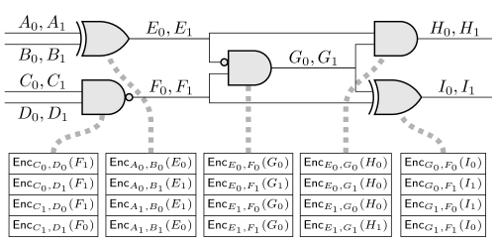
\includegraphics[width=1.0\textwidth]{Chapter2/Figs/Raster/garbledCircuit}
  \caption{Garbled Circuit example}
  \label{fig:garbledCircuit}
\end{figure}

Recent works provides optimizations to improve computation and communication
overhead associated with encrypt/decrypt operations and ciphertext tables'
sizes. In \cite{kolesnikov2008improved30}, the authors proposed a modification to
allow XOR gates to be evaluated \textit{for free}: the labels of XOR gates are
not chosen independently but by \(\omega_{i,0} = \omega_{i,1} \xor r\), for some
random value of \(r\). Pinkas et al. \cite{pinkas2009secure38} introduced a way to reduce communication size of binary gates by 25\%: each gate can be specified by three ciphertexts instead of all four. Finally, \cite{kolesnikov2009improved29} improve some commonly used circuits such as addition, comparision, etc. by reducing the number of non-XOR gates.

\subsection{Oblivious Transfer}
\label{sec:obliviousTransferPre}

\textit{"You take the blue pill, the story ends. You wake up in your bed and
  believe whatever you want to believe. You take the red pill, you stay in
  wonderland, and I show you how deep the rabbit hole goes."} - Morpheus to Neo,
the Matrix.


\begin{figure}[htbp!] 
\centering    
\includegraphics[width=1.0\textwidth]{Chapter2/Figs/Raster/RedPillBluePill}
\caption[Minion]{Red Pill - Blue Pill}
\label{fig:RedPillBluePill}
\end{figure}

What if, in such situation, there is a protocol to give privacy to
\(Neo\): \(Morpheus\) should not learn about \(Neo\)'s selection. Moreover, the
protocol can also provide privacy to \(Morpheus\): \(Neo\) should not learn
anything about the unchosen pill. In cryptography, Oblivious Transfer (OT) is a
protocol that can support such scenario. 
In the most basic form, it is a
two-parties protocol between a \textit{Sender} and a \textit{Receiver}, denoted
by \(\begin{psmallmatrix} 2 \\ 1 \end{psmallmatrix} \)-OT. The \(Sender\) uses
two private inputs \(x_{0}, x_{1}\) and the \(Receiver\) uses one input bit
\(s\). At the completion of the protocol, the \(Receiver\) gets the bit
\(x_{s}\) without letting the \(Sender\) know any information about the value of
\(s\): \(\begin{psmallmatrix} 2 \\ 1 \end{psmallmatrix}
\)-OT\((x_{0},x_{1};s) = x_{s}\).

The general idea is, when the receiver requests an item, the sender sends all the
items to the receiver and therefore it does not know which item is the one
requested. However, the response is encrypted in such a way that the receiver
can only decrypt the one he requested. A concrete implementation example of
\(\begin{psmallmatrix} 2 \\ 1 \end{psmallmatrix} \)-OT protocol based on
discrete log DH is illustrated in figure \ref{fig:DH21OT}. The receiver picks \(h_{0},h_{1}\) such that \(h_{0}h_{1} = h\), he cannot know both \(\log_{g}h_{0}\) and \(\log_{g}h_{1}\). Given \(h_{0}, h_{1}\), the sender returns ElGamal encryptions of bits \(x_{0}, x_{1}\) using \(h_{0},h_{1}\) as public keys. The receiver then decrypts one of the encryption to recover either \(x_{0} or x_{1}\)

\begin{figure}[h!]
  \centering
  \begin{equation*}
    \begin{array}{c c c}
      \text{\textbf{Sender}} & & \text{\textbf{Receiver}} \\
      \\
      (x_{0}, x_{1} \in \{0,1\}) & & (s \in \{0,1\}) \\
                             & & u \randomsample \mathbb{Z}_{n}\\
                             & & h_{s} \gets g^{u}\\
                             & & h_{1-s} \gets h/g^{u}\\
                             & \xleftarrow{h_{0}, h_{1}} & \\
      u_{0}, u_{1} \randomsample \mathbb{Z}_{n} & & \\
      (A_{0}, B_{0}) \gets (g^{u_{0}}, h_{0}^{u_{0}}g^{x_{0}}) & & \\
      (A_{1}, B_{1}) \gets (g^{u_{1}}, h_{1}^{u_{1}}g^{x_{1}}) & & \\
                             & \xrightarrow{(A_{0}, B_{0}),(A_{1}, B_{1})} & \\
      & & x_{s} \gets \log_{g}(B_{s}/A_{s}^{u})
    \end{array}
  \end{equation*}
  \caption{OT protocol based on DH}
  \label{fig:DH21OT}
\end{figure}

Efficient implementations of Oblivious Transfer can be found from \cite{naor2001efficient35}. The techniques from \cite{ishai2003extending24} can reduce a large number of OT protocol executions to \(\lambda\), where \(\lambda\) is the security parameter. In this thesis, we propose a new OT technique to be used with lattice-based cryptosystem.

\section{The Syntax and Security model}
\label{sec:syntaxModel}
We first describe the protocol and its security model in generic form.  We then can use them as a framework to apply and
analyze in our specific proposal.

% \subsubsection{Desirable properties}
% \label{sec:privacyProps}
% According to \cite{jain201650}, a secure template solution to biometric authentication should satisfy the following
% properties
% \begin{description}
% \item[Non-invertibility:] It is computationally hard to rebuild the original template from the encrypted one.
% \item[Non-linkability (Revocability):] It should be possible to revoke and to re-issue new encrypted templates using a
%   new key when the database is compromised.
% \item[Discriminability:] The secure scheme should not degrade the accuracy of the biometric authentication system.
% \end{description}
\subsubsection{The threats}
\label{sec:privacyReqs}
There are common security threats to many authentication systems such as Trojan horse, replay, man-in-the-middle (MITM)
attack, etc. Biometrics authentication systems are also vulnerable to such attacks. We can
borrow ideas from secure password-based schemes to address such issues. However, there are two categories of
vulnerabilities that are specific to biometric systems.  The first one is impersonation, or spoofing, the attack happens
at the client side where the adversary tries to cheat the system with counterfeit or invalid inputs.  The other issue is
at the server side with the privacy concern.

We will discuss the formal models that capture all the known threats of biometric authentication:
\begin{itemize}
\item Confidential data leakage due to attacks on the template database: Server breaches of biometric data always have
  catastrophic consequences (\cite{OPMsays563:online}), as we cannot change our fingerprints as easily as changing our
  passwords.
\item Hill-Climbing attack from the server side: This is also a privacy threat where the server trying to compute good
  inputs $X$ from the distance information between $X$ and $Y$ (\cite{uludag2004attacks}, \cite{higo2015privacy}). Note
  that Hill-Climbing attack by the client is very limited due to the limitation of the number of false authentication
  attempts in almost every biometric authentication system.
\item Impersonation by malicious client when the secret key of the user is known (replay attack): This happens when an
  attacker has access to the user's device but not his biometric, for example, in stolen device
  scenarios.(\cite{zhang2015fingerprints})
\item Impersonation by malicious client when the biometric template of the user is known (spoofing attack): This happens
  when an attacker collects biometric data and tries to reconstruct the template for authentication, for example,
  rebuilding the fingerprint from captured photos (\cite{zhang2015fingerprints},\cite{feng2011fingerprint}).
\item Cross matching of biometric data among databases: This threat uses information of the same user from different
  compromised databases to reconstruct the biometric template.
\end{itemize}

\subsubsection{The Generic Two-party model}

\begin{description}
\item[Entities:] There can be 2 or 3 typical entities involved in a secure biometric authentication system. The user
  $\mathcal{U}$, an authentication server $\mathcal{S}$, and a decryptor, who is a third party trusted by both of the
  users and the server. The decryptor presents in some systems (\cite{mandal2015comprehensive},
  \cite{hirano2013cryptographically}, \cite{higo2015privacy}), with the assumption that there is no collusion between
  this entity and $\user$ or $\server$. In our work, we aim to avoid the assumption of trusted decryptor party, so we
  only have two parties, $\user$ and $\server$.
\item[Biometrics Features in non-private setting] In biometric authentication systems (e.g., fingerprint authentication
  system), a user $\mathcal{U}$ first
  enrolls his fingerprint template $X$ with the server $\mathcal{S}$. $\mathcal{U}$ later authenticates with
  $\mathcal{S}$ using the same finger with a template $Y$, $\server$ uses an algorithm $Verify(X,Y)$ to obtain the
  result of the authentication: \textbf{Accept} or \textbf{Reject}. Different fingerprint system might use different
  features of fingers such as minutia or fingercode to compute this distance $\Delta$ between $X$ and $Y$ in the
  algorithm $Verify$. The distance $\Delta$ is compared to some predifined threshold value $\tau$ to determine the
  result of the authentication. We refer the reader to \cite{jain2007handbook} for biometric feature extraction and
  comparison techniques.\\

  Unlike password based system where $\user$ always uses one same query for many authentication, all biometric systems
  have the concept of False Acceptance Rate (FAR), where the system \textbf{Accept} an incorrect template; and False
  Rejection Rate (FRR), where the system \textbf{Reject} a genuine one.  Balancing these 2 rates while keeping good
  performances is one of the main challenges that fingerprint verification algorithms \cite{FVConGoi2:online} are trying
  to solve. We also reflect these two rates in our models.

\item[Algorithms and Procedures in privacy-preserving setting:] We describe the high level constructions of the protocol
  as follows
  \begin{description}
  \item[Enroll:] This procedure inserts records into the server's database.
    \begin{itemize}
    \item Input: Client: identity $k$, a registered template $X_k$; Server: Parameters of the cryptographic tools used.
    \item Output: A public-private key pair $(sk_k, pk_k)$ for the user $\user_k$. The server learns the protected
      template of $T_k$ of $X_k$.
    \end{itemize}
  \item[Auth:] This procedure allows a user to authenticate with the system.
    \begin{itemize}
    \item Input: Client: identity $k$, a query template $Y_k$ and the secret key $sk_k$; Server: record $(k, T_k, pk_k)$
    \item Output: The server learns the authentication result $res=\{\textbf{Accept,Reject}\}$
    \end{itemize}

  \item[Correctness Requirement:] A genuine user $\user_k$ does $(sk_k, T_k) \gets \mathbf{Enroll}(k, X_k)$ using a
    $X_k \in Supp(D_k)$ and later uses his biometric template $Y_k \randomsample D_k$ to do
    $$res \gets \mathbf{Auth}( (k, Y_k, sk_k), (k, T_k, pk_k))$$
    The privacy-preserving protocol works correctly if FRR under this system is exactly equal to FRR of the non-privacy
    preserving system:
    \[
      Pr[res = verify(X_k,Y_k)] = 1
    \]
  \end{description}
\end{description}

\subsubsection{The security model}
\begin{description}
\item[Privacy against an Honest But Curious server:] The security model is defined in terms of following security games.
  % Although the model assumes the server behaves honestly \emph{within} the protocol (since we our main aim is security
  % against passive exposure of server contents), it does allow the server to adversarially choose the client's
  % \emph{input} query templates $Y_i$ to try to learn about the attacked user's template $X_k$, so our model implies
  % security against `hill climbing attacks'~\cite{adler2005vulnerabilities}.

\item[The real game $\mathbf{Real}_{\attacker}(D_k,X_k)$:] This is the game for a privacy attack against the
  privacy-preserving protocol for the underlying biometric system, between an attacker $\attacker$ and a challenger
  $\challenger$. The input the game is an attacked $\user_k$ biometric distribution $D_k \in D_{bio}$ and a user
  template $X_k \in Supp(D_k)$.
  \begin{enumerate} %$\challenger$ selects a $\user_k$ with $D_k \in D_{bio}$ . For any $X_k \in Supp(D_k)$,
  \item $\challenger$ runs $(T_k, sk_k) \gets \mathbf{Enrol}(k,X_k)$ and sends $T_k$ to $\attacker$.
  \item For $i = 1 \dots q$:
    \begin{itemize}
    % \item $\attacker$ chooses and sends $Y_i$ to $\challenger$
    \item $\challenger$ samples \(Y_{i} \randomsample D_{k}\)
    \item $\challenger$ simulates the \textbf{Auth} protocol, playing the roles of both the client and the server:
      \[
        res \gets \mathbf{Auth_i}((k, Y_i, sk_k), (k, T_k, pk_k))
      \]
    \item Let $V_i$ denotes the $i^{th}$ view of $\server$ when $\challenger$ runs $\mathbf{Auth_i}$. $\challenger$
      sends the view $V_i$ to $\attacker$.
    \end{itemize}
  \item $\attacker$ outputs a bit $\beta$, representing some information that $\attacker$ has learned about
    $(D_k,X_k)$. The game output is $\mathbf{Real}_{\attacker}(D_k,X_k) = \beta$.
  \end{enumerate}

\item[The ideal game $\mathbf{Ideal}_{\attacker'}(D_k,X_k)$:] This is the game for a privacy attack against an ideal
  privacy scenario for the underlying biometric authentication system, where the attacker $\attacker'$ interacts with a
  challenger $\challenger'$. The input the game is an attacked $\user_k$ biometric distribution $D_k \in D_{bio}$ and a
  user template $X_k \in Supp(D_k)$. In this ideal game, the information $\attacker'$ can learn about $(D_k,X_k)$ is the
  value of \(HD_{X_{k}, Y_{k}}\) and the bit $Verify(X_k,Y_i)$.
  \begin{enumerate}
  \item For $i = 1 \dots q$:
    \begin{itemize}
    \item $\attacker'$ chooses query template $Y_i \in \{0,1\}^n$ and send it to $\challenger'$.
    % \item $\challenger'$ computes $res_i = verify(X_k, Y_i) \in \{\mathbf{Accept},\mathbf{Reject}\}$.
    \item $\challenger'$ sends $HD_{X,Y_{i}}$ to $\attacker'$.
    \end{itemize}
  \item $\attacker'$ output a bit $\beta'$, representing some information that $\attacker'$ has learned about
    $(D_k,X_k)$. The game output is $\mathbf{Ideal}_{\attacker'}(D_k,X_k) = \beta'$.
  \end{enumerate}
\end{description}
\begin{definition}
  [Privacy Security against Server] We say that a biometric authentication protocol is $q$-private in the sense of
  biometric template privacy against an honest but curious server $\server$ if for every efficient real-game attacker
  $\attacker$, there exists an efficient ideal-game attacker $\attacker'$ such that, for all $(D_k,X_k)$ we have:
  \[
    |\Pr[\mathbf{Real}_{\attacker}(D_k,X_k) = 1] - \Pr[\mathbf{Ideal}_{\attacker'}(D_k,X_k) = 1]| \leq negl(\lambda).
  \]
\end{definition}

\begin{description}
\item[Security against the malicious client:] In this work, we aim for security against active client, where an attacker
  $\attacker$ is assumed not to follow the protocol transcript.
  \begin{description}
  \item[Biometric Impersonation:] FAR is the usual biometric impersonation probability, it is inherent to the biometrics
    themselves without any cryptographic protocols. We first discuss this security game (which will be refered to as
    \textit{biometric impersonation}), then we elaborate the discussion to the models with privacy-preserving
    requirements.
    \begin{description}
    \item[Setup:] $\challenger$ samples $X_k \randomsample D_{k}$ from a random $\user_k$ ($D_k \randomsample D_{bio}$).
    \item[Query:] $\attacker$ is given access to the authentication oracle $verify(X_k,Y)$ that returns the
      authentication result of $\user_k$ with a query template $Y$. $\attacker$ has $q$ attempts to make queries, in
      each attempt, $\attacker$ chooses a $Y_{q}$ by himself and does $verify(X_k,Y_{q})$.
    \item[Guess:] $\attacker$ outputs $Y_{q'}$ such that $verify(X_k,Y_{q'}) = \textbf{Accept}$.
    \end{description}
    The advantage of $\attacker$ in the game is defined as
    \[
      \textbf{Adv}^{bio}_\attacker(\lambda) = Pr[verify(X_k,Y_{q'}) = \mathbf{Accept}]
    \]
    In this basic model, when $q=1$, the advantage of $\attacker$ is $FAR$.  In other words, we can say the advantage of
    $\attacker$ is $ \textbf{Adv}^{bio}_\attacker(\lambda) \leq q\times FAR$.

  \item[Privacy-Preserving Protocol:] This model extend the above protocol and captures the client side attacks
    mentioned in section \ref{sec:privacyReqs}.
    \begin{description}
    \item[Setup:] The setup phase includes 2 steps:
      \begin{itemize}
      \item $\challenger$ samples $X_k \randomsample D_{k}$ from a random $\user_k$ ($D_k \randomsample D_{bio}$).
      \item $\challenger$ runs $\textbf{Enroll}(k, X_k)$ that returns $(sk_k, T_k)$.
      \end{itemize}
    \item[Query:] In the query phase:
      \begin{itemize}
      \item $\attacker$ is given access to the authentication oracle $\mathbf{Auth}(Y)$ that returns the authentication
        result of $\user_k$ with a query template $Y$.
      \item $\attacker$ chooses the attack type $t \in \{I,II\}$ which specifies the scenario of key exposed or template
        exposed.

      \item $\challenger$ gives $sk_k$ if $t = I$ or $T_k$ if $t = II$ to $\attacker$. Note that, this model reflects
        the 2-factors authentication (the secret key and the biometric template), if $\attacker$ requests both factors,
        he loses the game.
      \item $\challenger$ and $\attacker$ runs $\mathbf{Auth()}$ $q$ times, For the $i^{th}$ run, $\attacker$ plays the
        client's role that chooses and sends $Y_i$ to $\challenger$, $\challenger$ plays the server's role that replies
        with $res_i = \mathbf{Auth}(Y_i)$.
      \end{itemize}
    \item[Guess:] $\attacker$ wins the game if it outputs $Y$ such that $\mathbf{Auth}(Y) = \textbf{Accepted}$.
    \end{description}
    The advantage of $\attacker$ in this game is defined as
    \[
      \textbf{Adv}^{Imp}_\attacker(\lambda) = Pr[\attacker \ wins] \
    \]
    We would want this advantage value not to be too large compared to the non-privacy-preserving biometric
    impersonation model's advantage $\textbf{Adv}^{bio}_\attacker(\lambda)$, which was bounded by $q \times FAR$.

  \end{description}

\end{description}
\begin{definition}
  [Impersonation Security] We say that a biometric authentication protocol is c-secure in the sense of template
  protection against the malicious user $\user$ if $\textbf{Adv}^{Imp}_\attacker(\lambda)$ is not greater than
  $\textbf{Adv}^{bio}_\attacker(\lambda)$ in some factor $c$ (if $c = 1$ we would have perfectly the same security level
  as the non-privacy-preserving system):
  \[\textbf{Adv}^{Imp}_\attacker(\lambda) \leq c \times \textbf{Adv}^{bio}_\attacker(\lambda)\]
\end{definition}


\section{Conclusion}
%%% Local Variables:
%%% mode: latex
%%% TeX-master: "../thesis"
%%% End: